\documentclass{../../kalkulus-ppt}

\author[Tetew]{Teosofi Hidayah Agung}
\date{\today}
\title[Kalkulus 2 - Bab 6]{Barisan dan Deret}
\institute[Matematika ITS]{Departemen Matematika\\ Institut Teknologi Sepuluh Nopember}
\titlegraphic{{\includegraphics[scale=0.3]{ITS.png}$\quad$\includegraphics[scale=0.02]{M.png}}}

\setbeamertemplate{itemize items}[circle]
\usetikzlibrary{arrows.meta}
\tikzset{
    kurva/.style={HIMAtua,very thick},
    pembanding/.style={teal!80!black,thick},
    bantu/.style={gray!85!black,densely dashed},
    sumbu/.style={-{Stealth[length=2mm]},gray!85!black},
    label grafik/.style={font=\scriptsize,inner sep=2pt}
}
\pgfplotsset{
    bidang/.style={
        width=6.05cm,height=4.15cm,axis lines=middle,
        samples=71,tick label style={font=\scriptsize},
        label style={font=\small},clip mode=individual
    },
    suku/.style={only marks,mark=*,mark size=1.65pt,HIMAtua}
}

\begin{document}

\begin{frame}
    \titlepage
\end{frame}

\begin{frame}{Daftar isi}
    \tableofcontents
\end{frame}

% Kalkulus 2 Bab 6.pdf, subbab 6.1.
\section{Barisan Takhingga}

\begin{frame}{\insertsection}
    \framesubtitle{Setiap bilangan bulat positif menunjuk satu suku}
    \begin{columns}[c,onlytextwidth]
        \begin{column}{.52\textwidth}
            \begin{definisi}[Barisan takhingga]
                Barisan real adalah fungsi dari bilangan bulat
                positif ke $\R$. Nilai pada indeks $n$ disebut suku
                ke-$n$ dan ditulis $a_n$. Notasinya
                \[
                    \{a_n\}_{n=1}^{\infty}
                    \quad\text{atau}\quad a_1,a_2,a_3,\ldots.
                \]
            \end{definisi}
            Urutan suku ditentukan oleh indeksnya. Jika indeks
            dimulai dari $0$, tulis $\{a_n\}_{n=0}^{\infty}$.
        \end{column}
        \begin{column}{.44\textwidth}
            \begin{contoh}
                Pada $\{3^n\}_{n=1}^{\infty}$, lima suku awalnya
                $3,9,27,81,243$. Mulai dari $n=0$ akan memberi
                suku awal $3^0=1$.
            \end{contoh}
            \onslide<2->{Tanda berselang dapat dimuat dalam rumus.
            Misalnya, $a_n=(-1)^{n+1}\frac{n+1}{n+2}$ memberi
            \[
                \frac23,\ -\frac34,\ \frac45,\ -\frac56,\ldots.
            \]}
        \end{column}
    \end{columns}
\end{frame}

\begin{frame}{\insertsection}
    \framesubtitle{Grafik barisan berupa titik pada indeks bulat}
    \begin{columns}[c,onlytextwidth]
        \begin{column}{.49\textwidth}
            \begin{contoh}
                Uraikan dan gambarkan $a_n=2/n^2$ untuk $n\ge1$.
            \end{contoh}
            \onslide<2->{Suku awalnya adalah
            \[
                2,\quad \frac12,\quad\frac29,\quad\frac18,\ldots.
            \]
            Titik $(n,a_n)$ dapat dibaca dari kurva $f(x)=2/x^2$
            yang dievaluasi pada $x=n$. Kurva putus-putus
            memperlihatkan fungsi real yang menaungi titik-titik itu.}
        \end{column}
        \begin{column}{.47\textwidth}
            \centering
            \begin{tikzpicture}
                \begin{axis}[bidang,xmin=0,xmax=7.65,ymin=0,ymax=2.52,
                    xlabel={$n$},ylabel={$a_n$},xtick={1,...,7},
                    ytick={.5,1,2},yticklabels={$1/2$,$1$,$2$}]
                    \only<2->{\addplot[bantu,domain=.93:7.3] {2/x^2};}
                    \addplot[suku,domain=1:7,samples=7] {2/x^2};
                \end{axis}
            \end{tikzpicture}
        \end{column}
    \end{columns}
\end{frame}

\begin{frame}{\insertsection}
    \framesubtitle{Empat perilaku yang tampak saat indeks membesar}
    \centering
    \begin{tikzpicture}
        \begin{axis}[bidang,width=3.24cm,height=3.23cm,
            xmin=0,xmax=9,ymin=0,ymax=10.15,xtick={1,8},ytick={2,9},
            title={$a_n=n+1$},title style={font=\small}]
            \addplot[suku,domain=1:8,samples=8] {x+1};
        \end{axis}
        \begin{axis}[bidang,at={(3.65cm,0)},anchor=south west,
            width=3.24cm,height=3.23cm,
            xmin=0,xmax=9,ymin=-1.4,ymax=1.4,xtick={1,8},ytick={-1,1},
            title={$a_n=(-1)^n$},title style={font=\small}]
            \addplot[suku] coordinates {(1,-1) (2,1) (3,-1) (4,1)
                (5,-1) (6,1) (7,-1) (8,1)};
        \end{axis}
        \begin{axis}[bidang,at={(7.3cm,0)},anchor=south west,
            width=3.24cm,height=3.23cm,
            xmin=0,xmax=9,ymin=0,ymax=1.22,xtick={1,8},ytick={1},
            title={$a_n=\frac{n}{n+2}$},title style={font=\small}]
            \addplot[bantu,domain=0:9] {1};
            \addplot[suku,domain=1:8,samples=8] {x/(x+2)};
        \end{axis}
        \begin{axis}[bidang,at={(10.95cm,0)},anchor=south west,
            width=3.24cm,height=3.23cm,
            xmin=0,xmax=9,ymin=0,ymax=1.42,xtick={1,8},ytick={1},
            title={$a_n=1+\frac{(-1)^n}{2n}$},title style={font=\small}]
            \addplot[bantu,domain=0:9] {1};
            \addplot[suku,domain=1:8,samples=8] {1+cos(180*x)/(2*x)};
        \end{axis}
    \end{tikzpicture}\par
    \smallskip
    \onslide<2->{\small
        Dua barisan pertama divergen. Dua barisan terakhir menuju $1$,
        masing-masing dari bawah dan dengan osilasi yang mengecil.
        Pada $(-1)^n$, suku genap dan ganjil menuju dua nilai yang berbeda.}
\end{frame}

\begin{frame}{\insertsection}
    \framesubtitle{Seluruh suku di ekor barisan harus masuk ke pita $\varepsilon$}
    \begin{columns}[c,onlytextwidth]
        \begin{column}{.53\textwidth}
            \begin{definisi}[Konvergensi barisan]
                Ditulis $\lim_{n\to\infty}a_n=L$ jika untuk
                setiap $\varepsilon>0$, ada bilangan bulat positif
                $N$ sehingga
                \[
                    n\ge N\quad\Longrightarrow\quad |a_n-L|<\varepsilon.
                \]
                Barisan tanpa limit berhingga disebut divergen.
            \end{definisi}
            $N$ boleh bergantung pada $\varepsilon$. Pita yang
            semakin sempit biasanya memerlukan $N$ yang lebih besar.
        \end{column}
        \begin{column}{.43\textwidth}
            \centering
            \begin{tikzpicture}
                \begin{axis}[bidang,width=5.7cm,xmin=0,xmax=14,
                    ymin=0,ymax=1.41,xlabel={$n$},ylabel={$a_n$},
                    xtick={1,4,9,13},xticklabels={$1$,$4$,$N=9$,$13$},
                    ytick={.8,1,1.2},yticklabels={$L-\varepsilon$,$L$,$L+\varepsilon$}]
                    \fill[HIMAmuda!22] (axis cs:0,.8) rectangle (axis cs:13.75,1.2);
                    \addplot[bantu,domain=0:13.75] {.8};
                    \addplot[pembanding,domain=0:13.75] {1};
                    \addplot[bantu,domain=0:13.75] {1.2};
                    \draw[bantu] (axis cs:8.5,0) -- (axis cs:8.5,1.2);
                    \addplot[suku,domain=1:13,samples=13] {x/(x+2)};
                    \addplot[suku,teal!80!black,domain=9:13,samples=5] {x/(x+2)};
                \end{axis}
            \end{tikzpicture}\par
            \small Untuk $a_n=n/(n+2)$ dan $\varepsilon=1/5$,
            semua suku mulai $n=9$ berada di dalam pita.
        \end{column}
    \end{columns}
\end{frame}

\begin{frame}{\insertsection}
    \framesubtitle{Mencari $N$ dari besar galat yang diizinkan}
    \begin{columns}[c,onlytextwidth]
        \begin{column}{.47\textwidth}
            \begin{contoh}
                Buktikan $\displaystyle\lim_{n\to\infty}
                \frac{n}{n+2}=1$ dengan definisi.
            \end{contoh}
            \onslide<2->{Jarak suku ke calon limit adalah
            \[
                \left|\frac{n}{n+2}-1\right|=\frac{2}{n+2}.
            \]
            Untuk membuat jarak ini kurang dari $\varepsilon$,
            cukup pastikan $n>2/\varepsilon-2$.}
        \end{column}
        \begin{column}{.49\textwidth}
            \onslide<3->{%
                \begin{block}{Pilih satu indeks pemotong}
                    Ambil $N$ bulat positif dengan
                    $N>2/\varepsilon-2$. Maka untuk seluruh $n\ge N$,
                    \[
                        \frac{2}{n+2}\le\frac{2}{N+2}<\varepsilon.
                    \]
                \end{block}
                Misalnya, $\varepsilon=1/20$ memberi syarat $N>38$.
                Kita dapat memakai $N=39$.
            }
        \end{column}
    \end{columns}
\end{frame}

\begin{frame}{\insertsection}
    \framesubtitle{Operasi aljabar pada barisan yang sudah konvergen}
    \begin{columns}[c,onlytextwidth]
        \begin{column}{.51\textwidth}
            \begin{teorema}[Sifat limit barisan]
                Jika $a_n\to A$, $b_n\to B$, dan $c$ konstanta,
                \[
                    \begin{aligned}
                        \lim c&=c,& \lim ca_n&=cA,\\
                        \lim(a_n\pm b_n)&=A\pm B,&
                        \lim a_nb_n&=AB,\\
                        \lim\frac{a_n}{b_n}&=\frac AB&& (B\ne0).
                    \end{aligned}
                \]
            \end{teorema}
            Syarat $B\ne0$ memastikan $b_n$ jauh dari nol
            untuk semua $n$ yang cukup besar.
        \end{column}
        \begin{column}{.45\textwidth}
            \begin{contoh}
                Tentukan limit $\{(3n-1)/(2n+5)\}$.
            \end{contoh}
            \onslide<2->{Bagi pembilang dan penyebut dengan $n$.
            \[
                \lim_{n\to\infty}\frac{3-1/n}{2+5/n}=\frac32.
            \]
            Pembilang menuju $3$, penyebut menuju $2$, sehingga
            aturan hasil bagi berlaku.}
        \end{column}
    \end{columns}
\end{frame}

\begin{frame}{\insertsection}
    \framesubtitle{Limit fungsi real dapat dipakai pada suku berindeks bulat}
    \begin{columns}[c,onlytextwidth]
        \begin{column}{.47\textwidth}
            \begin{block}{Dari fungsi ke barisan}
                Jika $a_n=f(n)$ untuk $n$ yang cukup besar
                dan $\lim_{x\to\infty}f(x)=L$, maka $a_n\to L$.
                Setelah semua $x$ yang cukup besar masuk ke
                pita limit, semua bilangan bulat di bagian itu juga masuk.
            \end{block}
            Diferensiasi dalam aturan L'Hôpital dilakukan
            terhadap variabel real $x$ pada fungsi $f$.
        \end{column}
        \begin{column}{.49\textwidth}
            \begin{contoh}
                Hitung $\displaystyle\lim_{n\to\infty}\frac{n^2}{e^n}$.
            \end{contoh}
            \onslide<2->{Untuk $f(x)=x^2/e^x$, terapkan
            aturan L'Hôpital dua kali.
            \[
                \lim_{x\to\infty}\frac{x^2}{e^x}
                =\lim_{x\to\infty}\frac{2x}{e^x}
                =\lim_{x\to\infty}\frac{2}{e^x}=0.
            \]
            Nilai $f(n)$ mewarisi limit $0$ tersebut.}
        \end{column}
    \end{columns}
\end{frame}

\begin{frame}{\insertsection}
    \framesubtitle{Dua pembatas dengan limit sama mengapit barisan}
    \begin{columns}[c,onlytextwidth]
        \begin{column}{.51\textwidth}
            \begin{teorema}[Teorema apit]
                Jika $a_n\le b_n\le c_n$ untuk semua $n$ yang
                cukup besar dan $a_n,c_n\to L$, maka $b_n\to L$.
            \end{teorema}
            \begin{contoh}
                Untuk $b_n=\cos n/(n+1)$,
                \[
                    -\frac1{n+1}\le b_n\le\frac1{n+1}.
                \]
            \end{contoh}
            \onslide<2->{Kedua batas menuju $0$, sehingga
            osilasi $b_n$ juga menyempit menuju $0$.}
        \end{column}
        \begin{column}{.45\textwidth}
            \centering
            \begin{tikzpicture}
                \begin{axis}[bidang,xmin=0,xmax=14.7,ymin=-.56,ymax=.56,
                    xlabel={$n$},ylabel={$b_n$},xtick={1,4,8,12},
                    ytick={-.5,.5},yticklabels={$-1/2$,$1/2$}]
                    \addplot[pembanding,domain=1:14] {1/(x+1)};
                    \addplot[pembanding,domain=1:14] {-1/(x+1)};
                    \addplot[suku,domain=1:14,samples=14] {cos(deg(x))/(x+1)};
                \end{axis}
            \end{tikzpicture}
        \end{column}
    \end{columns}
\end{frame}

\begin{frame}{\insertsection}
    \framesubtitle{Kemonotonan bisa diperiksa dari dua suku berurutan}
    \begin{columns}[T,onlytextwidth]
        \begin{column}{.49\textwidth}
            \begin{definisi}[Barisan monoton]
                Bandingkan $a_n$ dan $a_{n+1}$ untuk semua $n$.
                \[
                    \begin{array}{l|l}
                        \text{Naik} & a_{n+1}>a_n\\
                        \text{Tidak turun} & a_{n+1}\ge a_n\\
                        \text{Turun} & a_{n+1}<a_n\\
                        \text{Tidak naik} & a_{n+1}\le a_n
                    \end{array}
                \]
                Barisan tidak turun atau tidak naik disebut monoton.
                Barisan naik atau turun disebut monoton ketat.
            \end{definisi}
            Contoh tidak turun ialah $1,1,2,2,3,3,\ldots$.
        \end{column}
        \begin{column}{.47\textwidth}
            \begin{block}{Selisih dan rasio}
                Periksa tanda $a_{n+1}-a_n$. Jika setiap
                $a_n>0$, bandingkan $a_{n+1}/a_n$ dengan $1$.
            \end{block}
            \begin{contoh}
                Untuk $a_n=n/(n+2)$, diperoleh
                \[
                    a_{n+1}-a_n=\frac{2}{(n+2)(n+3)}>0.
                \]
                Rasionya $1+2/[n(n+3)]>1$.
                Keduanya menunjukkan barisan naik.
            \end{contoh}
        \end{column}
    \end{columns}
\end{frame}

\begin{frame}{\insertsection}
    \framesubtitle{Kemonotonan dapat mulai berlaku setelah beberapa suku}
    \begin{columns}[c,onlytextwidth]
        \begin{column}{.53\textwidth}
            \begin{definisi}[Monoton di akhir]
                Barisan disebut monoton di akhir jika ada $N$
                sehingga ekor $a_N,a_{N+1},\ldots$ monoton.
            \end{definisi}
            \begin{contoh}
                Tentukan kapan $a_n=5^n/n!$ mulai turun.
            \end{contoh}
            \onslide<2->{%
                \[
                    \frac{a_{n+1}}{a_n}=\frac{5}{n+1}<1
                    \quad\text{bila } n\ge5.
                \]
                Suku ke-$4$ sama dengan suku ke-$5$ karena
                rasionya $1$ pada $n=4$. Ekor mulai $a_5$ turun.}
        \end{column}
        \begin{column}{.43\textwidth}
            \centering
            \begin{tikzpicture}
                \begin{axis}[bidang,width=5.75cm,
                    xmin=0,xmax=12.9,ymin=0,ymax=29.5,
                    xlabel={$n$},ylabel={$a_n$},xtick={1,4,5,8,12},
                    ytick={5,15,25}]
                    \addplot[suku] coordinates {(1,5) (2,12.5) (3,20.833)
                        (4,26.042) (5,26.042) (6,21.701) (7,15.501)
                        (8,9.688) (9,5.382) (10,2.691) (11,1.223) (12,.510)};
                    \only<2->{%
                        \draw[bantu] (axis cs:4.5,0) -- (axis cs:4.5,27.9);
                        \addplot[suku,teal!80!black] coordinates
                            {(5,26.042) (6,21.701) (7,15.501)
                             (8,9.688) (9,5.382) (10,2.691) (11,1.223) (12,.510)};
                    }
                \end{axis}
            \end{tikzpicture}
        \end{column}
    \end{columns}
\end{frame}

\begin{frame}{\insertsection}
    \framesubtitle{Barisan monoton memerlukan batas di arah geraknya}
    \begin{columns}[T,onlytextwidth]
        \begin{column}{.48\textwidth}
            \begin{teorema}[Barisan tidak turun]
                Jika $\{a_n\}$ tidak turun dan mempunyai batas
                atas, maka barisan konvergen ke batas atas terkecilnya.
                Jika tak berbatas atas, maka $a_n\to+\infty$.
            \end{teorema}
            Jika $L$ batas atas terkecil, ada $a_N>L-\varepsilon$.
            Untuk $n\ge N$ berlaku $L-\varepsilon<a_N\le a_n\le L$.
        \end{column}
        \begin{column}{.48\textwidth}
            \begin{teorema}[Barisan tidak naik]
                Jika $\{b_n\}$ tidak naik dan mempunyai batas
                bawah, maka barisan konvergen ke batas bawah terbesarnya.
                Jika tak berbatas bawah, maka $b_n\to-\infty$.
            \end{teorema}
            Pakai hasil di kiri pada $\{-b_n\}$, yang tidak turun
            bila $\{b_n\}$ tidak naik.
        \end{column}
    \end{columns}
    \smallskip
    \onslide<2->{%
        \begin{block}{Cukup periksa ekornya}
            Untuk $a_n=n/(n+2)$, sudah diperoleh bahwa $a_n$ naik
            dan $a_n<1$. Teorema menjamin limit ada. Nilainya
            diperoleh dari rumus limit atau diketahui dari batas atas terkecil.
        \end{block}
    }
\end{frame}

\begin{frame}{\insertsection}
    \framesubtitle{Untuk barisan rekursif, buktikan dulu limitnya ada}
    \begin{columns}[T,onlytextwidth]
        \begin{column}{.49\textwidth}
            \begin{contoh}
                Mulai dari $a_1=4$ dan
                $a_{n+1}=\frac12(a_n+9/a_n)$. Tentukan limitnya.
            \end{contoh}
            \onslide<2->{Identitas
            \[
                a_{n+1}-3=\frac{(a_n-3)^2}{2a_n}
            \]
            menunjukkan bahwa $a_n\ge3$ untuk semua $n$
            melalui induksi dari $a_1=4$.}
        \end{column}
        \begin{column}{.47\textwidth}
            \onslide<3->{Karena $a_n\ge3$,
            \[
                a_{n+1}-a_n=\frac{9-a_n^2}{2a_n}\le0.
            \]
            Barisan tidak naik dan berbatas bawah, jadi $a_n\to L$
            untuk suatu $L\ge3$.}
            \onslide<4->{Ambil limit pada relasi rekursif.
            \[
                L=\frac12\left(L+\frac9L\right)
                \quad\Longrightarrow\quad L^2=9.
            \]
            Dengan $L\ge3$, diperoleh $L=3$.}
        \end{column}
    \end{columns}
\end{frame}

\begin{frame}{\insertsection}
    \framesubtitle{Latihan limit, kemonotonan, dan batas}
    \begin{latihan}
        \begin{enumerate}
            \item Gunakan definisi untuk membuktikan $3/(n+1)\to0$.
            \item Tunjukkan bahwa $b_n=(4n+2)/(n+5)$ naik dan berbatas atas.
                Berapa limitnya?
            \item Tentukan limit $\{(-1)^n(2+1/n)\}$ jika ada.
        \end{enumerate}
    \end{latihan}
    \onslide<2->{%
        \begin{block}{Cek jawaban}
            \begin{enumerate}
                \item Ambil $N$ bulat positif dengan $N>3/\varepsilon-1$.
                \item $b_n=4-18/(n+5)<4$ dan $18/(n+5)$ turun, jadi $b_n$ naik.
                    Karena $18/(n+5)\to0$, limitnya $4$.
                \item Suku genap menuju $2$ dan suku ganjil menuju $-2$, jadi divergen.
            \end{enumerate}
        \end{block}
    }
\end{frame}

% Kalkulus 2 Bab 6.pdf, subbab 6.2.
\section{Deret Takhingga}

\begin{frame}{\insertsection}
    \framesubtitle{Suku deret adalah penambahan dari satu tahap ke tahap berikutnya}
    \begin{columns}[c,onlytextwidth]
        \begin{column}{.52\textwidth}
            \begin{definisi}[Deret takhingga]
                Deret dengan suku $u_1,u_2,\ldots$ ditulis
                \[
                    u_1+u_2+u_3+\cdots=\sum_{k=1}^\infty u_k.
                \]
                Ekspresi ini menyatakan penjumlahan bertahap.
                Nilai jumlahnya ditentukan melalui limit.
            \end{definisi}
            Pada ilustrasi Zeno, pelari menempuh setengah dari
            sisa lintasan setiap tahap. Untuk lintasan $2$ m,
            panjang tahapnya $1,\frac12,\frac14,\frac18,\ldots$ m.
        \end{column}
        \begin{column}{.44\textwidth}
            \centering
            \begin{tikzpicture}[x=.9cm,y=.85cm]
                \fill[HIMAmuda!32] (0,0) rectangle (3,.4);
                \fill[teal!38] (3,0) rectangle (4.5,.4);
                \fill[HIMAmuda!32] (4.5,0) rectangle (5.25,.4);
                \fill[teal!38] (5.25,0) rectangle (5.625,.4);
                \draw[kurva] (0,0) rectangle (6,.4);
                \foreach \x/\label in {0/0,3/1,4.5/{3/2},5.25/{7/4},6/2}
                    \draw[gray!85!black] (\x,-.1) -- (\x,.4)
                        node[pos=0,below,label grafik] {$\label$};
                \node[label grafik] at (1.5,.71) {tahap $1$};
                \node[label grafik] at (3.75,.71) {tahap $2$};
                \draw[sumbu] (0,-.55) -- (6.25,-.55)
                    node[below left,label grafik] {posisi (m)};
            \end{tikzpicture}\par
            \small Setelah $n$ tahap, sisa lintasannya $2^{1-n}$ m.
        \end{column}
    \end{columns}
\end{frame}

\begin{frame}{\insertsection}
    \framesubtitle{Konvergensi deret ditentukan oleh barisan jumlah parsial}
    \begin{columns}[c,onlytextwidth]
        \begin{column}{.51\textwidth}
            \begin{definisi}[Jumlah parsial dan jumlah deret]
                Tulis $S_n=\sum_{k=1}^{n}u_k$.
                Jika $S_n\to S$ dengan $S$ berhingga, deret
                konvergen dan $\sum_{k=1}^{\infty}u_k=S$.
                Jika $\{S_n\}$ divergen, deret juga divergen.
            \end{definisi}
            Untuk lintasan Zeno tadi,
            $S_n=2-2^{1-n}\to2$. Indeks $n$ menentukan
            banyaknya tahap yang sudah dijumlahkan.
        \end{column}
        \begin{column}{.45\textwidth}
            \centering
            \begin{tikzpicture}
                \begin{axis}[bidang,width=5.7cm,height=3.8cm,xmin=0,xmax=9,
                    ymin=0,ymax=2.35,xlabel={$n$},ylabel={$S_n$},
                    xtick={1,3,5,8},ytick={1,1.5,2},
                    yticklabels={$1$,$3/2$,$2$}]
                    \addplot[pembanding,dashed,domain=0:8.8] {2};
                    \addplot[suku,domain=1:8,samples=8] {2-2^(1-x)};
                \end{axis}
            \end{tikzpicture}\par
            \small Jarak ke $2$ mengecil setiap tahap.
        \end{column}
    \end{columns}
\end{frame}

\begin{frame}{\insertsection}
    \framesubtitle{Hitung beberapa jumlah parsial sebelum menilai deret}
    \begin{columns}[c,onlytextwidth]
        \begin{column}{.51\textwidth}
            \begin{contoh}
                Apakah $1-1+1-1+\cdots$ mempunyai jumlah?
            \end{contoh}
            \onslide<2->{Jumlah parsialnya
            \[
                S_1=1,\quad S_2=0,\quad S_3=1,\quad S_4=0.
            \]
            Untuk setiap $m\ge1$, $S_{2m-1}=1$ dan
            $S_{2m}=0$. Karena dua ekor indeks itu berbeda nilai,
            $\{S_n\}$ divergen.}
            \onslide<3->{Pengelompokan $(1-1)+(1-1)+\cdots$
            hanya mengamati $S_{2m}$, padahal definisi meminta
            limit melalui semua indeks.}
        \end{column}
        \begin{column}{.45\textwidth}
            \centering
            \begin{tikzpicture}
                \begin{axis}[bidang,width=5.75cm,height=3.75cm,
                    xmin=0,xmax=9,ymin=-.25,ymax=1.3,
                    xlabel={$n$},ylabel={$S_n$},
                    xtick={1,...,8},ytick={1}]
                    \only<2->{%
                        \addplot[suku] coordinates {(1,1) (3,1) (5,1) (7,1)};
                        \addplot[suku,teal!80!black] coordinates {(2,0) (4,0) (6,0) (8,0)};
                    }
                \end{axis}
            \end{tikzpicture}
        \end{column}
    \end{columns}
\end{frame}

\begin{frame}{\insertsection}
    \framesubtitle{Deret geometrik mempunyai rasio yang tetap}
    \begin{columns}[T,onlytextwidth]
        \begin{column}{.48\textwidth}
            \begin{teorema}[Deret geometrik]
                Untuk $a\ne0$, deret
                $a+ar+ar^2+\cdots$ konvergen tepat ketika $|r|<1$.
                Dalam kasus itu,
                \[
                    \sum_{k=0}^{\infty}ar^k=\frac{a}{1-r}.
                \]
            \end{teorema}
            Di sini $a$ suku pertama dan $r$ rasio antar suku.
            Jika $a=0$, setiap suku bernilai nol.
        \end{column}
        \begin{column}{.48\textwidth}
            \begin{block}{Cara mendapatkan rumus}
                Pengurangan $S_n-rS_n$ menyisakan dua suku.
                \[
                    \begin{aligned}
                        (1-r)S_n&=a-ar^n,\\
                        S_n&=\frac{a(1-r^n)}{1-r}\quad (r\ne1).
                    \end{aligned}
                \]
                Jika $|r|<1$, maka $r^n\to0$.
            \end{block}
            Untuk $r=1$, $S_n=na$. Untuk $r=-1$, $S_n$
            berselang antara $a$ dan $0$. Jika $|r|>1$,
            $|r|^n$ membesar tanpa batas.
        \end{column}
    \end{columns}
\end{frame}

\begin{frame}{\insertsection}
    \framesubtitle{Rasio negatif menghasilkan pendekatan dari dua sisi}
    \begin{columns}[c,onlytextwidth]
        \begin{column}{.53\textwidth}
            \begin{contoh}
                Hitung $6-2+\frac23-\frac29+\cdots$.
            \end{contoh}
            \onslide<2->{Suku pertama $6$ dan rasio $-1/3$.
            Karena $|r|=1/3<1$,
            \[
                S=\frac{6}{1+1/3}=\frac92.
            \]}
            \onslide<3->{Dari $S_n=\tfrac92[1-(-1/3)^n]$,
            suku $S_n$ berindeks ganjil di atas $9/2$
            dan indeks genap di bawahnya. Jarak ke limit
            mengecil dengan faktor $1/3$ setiap langkah.}
        \end{column}
        \begin{column}{.43\textwidth}
            \centering
            \begin{tikzpicture}
                \begin{axis}[bidang,width=5.7cm,xmin=0,xmax=8.8,
                    ymin=3.65,ymax=6.38,xlabel={$n$},ylabel={$S_n$},
                    xtick={1,2,4,6,8},ytick={4,4.5,6},
                    yticklabels={$4$,$9/2$,$6$}]
                    \only<2->{%
                        \addplot[pembanding,dashed,domain=0:8.5] {4.5};
                        \addplot[suku,domain=1:8,samples=8]
                            {4.5*(1-cos(180*x)*(1/3)^x)};
                    }
                \end{axis}
            \end{tikzpicture}
        \end{column}
    \end{columns}
\end{frame}

\begin{frame}{\insertsection}
    \framesubtitle{Desimal berulang dan pantulan sama-sama membentuk deret geometrik}
    \begin{columns}[T,onlytextwidth]
        \begin{column}{.47\textwidth}
            \begin{contoh}[Desimal berulang]
                Nyatakan $0{,}\overline{27}$ sebagai pecahan.
            \end{contoh}
            \onslide<2->{Pemisahan dua digit memberi
            \[
                \frac{27}{100}+\frac{27}{100^2}+\frac{27}{100^3}+\cdots.
            \]
            Gunakan $a=27/100$ dan $r=1/100$ untuk
            mendapatkan $S=27/99=3/11$.}
        \end{column}
        \begin{column}{.49\textwidth}
            \begin{contoh}[Lintasan bola]
                Bola jatuh dari $12$ m. Setiap pantulan
                mencapai sepertiga tinggi sebelumnya.
                Berapa total jarak vertikalnya?
            \end{contoh}
            \onslide<3->{Setelah jatuh pertama, tiap tinggi
            pantulan dihitung dua kali, saat naik dan turun.
            \[
                D=12+2(4+4/3+4/9+\cdots)=24\ \mathrm{m}.
            \]}
        \end{column}
    \end{columns}
\end{frame}

\begin{frame}{\insertsection}
    \framesubtitle{Pecahan parsial dapat menyingkap deret teleskopik}
    \begin{contoh}
        Tentukan jumlah $\displaystyle\sum_{k=1}^\infty \frac{2}{k(k+2)}$.
    \end{contoh}
    \onslide<2->{Gunakan $\frac{2}{k(k+2)}=\frac1k-\frac1{k+2}$.
    Untuk $n\ge5$, tulis jumlah parsial sebagai
    \[
        S_n=\left(1-\textcolor{teal!80!black}{\tfrac13}\right)
         +\left(\tfrac12-\textcolor{teal!80!black}{\tfrac14}\right)
         +\left(\textcolor{teal!80!black}{\tfrac13}-\tfrac15\right)
         +\left(\textcolor{teal!80!black}{\tfrac14}-\tfrac16\right)
         +\cdots+\left(\tfrac1n-\tfrac1{n+2}\right).
    \]}
    \onslide<3->{Setelah suku tengah saling menghapus, tersisa
    \[
        S_n=1+\frac12-\frac1{n+1}-\frac1{n+2}
        \quad\Longrightarrow\quad S=\frac32.
    \]}
\end{frame}

\begin{frame}{\insertsection}
    \framesubtitle{Konvergensi mengharuskan suku menuju nol}
    \begin{columns}[c,onlytextwidth]
        \begin{column}{.52\textwidth}
            \begin{teorema}[Uji divergensi suku ke-$n$]
                Jika $\sum_{n=1}^{\infty}u_n$ konvergen, maka
                $\lim_{n\to\infty}u_n=0$.
                Jika limit suku tak nol atau limitnya tidak ada,
                deret divergen.
            \end{teorema}
            Sebab $u_n=S_n-S_{n-1}$. Bila $S_n\to S$,
            kedua jumlah parsial menuju nilai yang sama dan
            selisihnya menuju $0$.
        \end{column}
        \begin{column}{.44\textwidth}
            \begin{contoh}
                Untuk $u_n=(2n+1)/(3n+2)$, limit sukunya
                $2/3$. Maka $\sum u_n$ divergen.
            \end{contoh}
            \onslide<2->{Jika $u_n\to0$, uji ini belum menentukan
            konvergensi. Deret $\sum 1/2^n$ konvergen, sementara
            $\sum 1/n$ divergen, walau kedua sukunya menuju nol.}
        \end{column}
    \end{columns}
\end{frame}

\begin{frame}{\insertsection}
    \framesubtitle{Deret harmonik terus bertambah walau sukunya mengecil}
    \begin{columns}[c,onlytextwidth]
        \begin{column}{.53\textwidth}
            \begin{block}{Deret harmonik}
                Deret $\displaystyle\sum_{k=1}^\infty \frac1k$
                disebut deret harmonik. Kelompokkan suku menurut
                indeks $2$, $3$--$4$, $5$--$8$, dan seterusnya.
            \end{block}
            Pada kelompok $2^{j-1}<k\le2^j$, ada $2^{j-1}$
            suku dan masing-masing paling kecil $1/2^j$.
            \onslide<2->{Jumlah setiap kelompok minimal $1/2$,
            sehingga $S_{2^m}\ge1+m/2$. Jumlah parsial tak terbatas,
            jadi deret divergen.}
        \end{column}
        \begin{column}{.43\textwidth}
            \centering
            \begin{tikzpicture}[x=.61cm,y=1.07cm]
                \draw[sumbu] (0,0) -- (8.62,0) node[right,label grafik] {$k$};
                \foreach \k in {1,...,8} {
                    \filldraw[fill=HIMAmuda!25,draw=HIMAtua]
                        ({\k-.26},0) rectangle ({\k+.26},{2.9/\k});
                    \node[below,label grafik] at (\k,0) {$\k$};
                }
                \draw<2->[pembanding] (1.74,1.45) -- (2.26,1.45)
                    node[midway,above,label grafik] {$1/2$};
                \draw<2->[pembanding] (2.74,.725) -- (4.26,.725)
                    node[midway,above right,label grafik] {$1/4$};
                \draw<2->[pembanding] (4.74,.3625) -- (8.26,.3625)
                    node[midway,above,label grafik] {$1/8$};
                \node[label grafik] at (1,3.14) {$1/k$};
            \end{tikzpicture}\par
            \small Tinggi batang menyatakan nilai suku.
        \end{column}
    \end{columns}
\end{frame}

\begin{frame}{\insertsection}
    \framesubtitle{Latihan memilih rumus atau uji divergensi}
    \begin{columns}[T,onlytextwidth]
        \begin{column}{.48\textwidth}
            \begin{latihan}
                Tentukan status konvergensinya. Jika konvergen,
                hitung jumlah deretnya.
                \begin{enumerate}
                    \item $\sum_{n=1}^\infty 4(\tfrac23)^{n-1}$.
                    \item $\sum_{n=1}^\infty
                        \bigl(\tfrac1{n+1}-\tfrac1{n+2}\bigr)$.
                    \item $\sum_{n=1}^\infty \tfrac{2n+1}{n+3}$.
                \end{enumerate}
            \end{latihan}
        \end{column}
        \begin{column}{.48\textwidth}
            \onslide<2->{%
                \begin{block}{Cek jawaban}
                    \begin{enumerate}
                        \item Geometrik, $S=4/(1-2/3)=12$.
                        \item Teleskopik, $S_n=\tfrac12-\tfrac1{n+2}\to\tfrac12$.
                        \item Divergen karena sukunya menuju $2$.
                    \end{enumerate}
                \end{block}
            }
        \end{column}
    \end{columns}
\end{frame}

% Kalkulus 2 Bab 6.pdf, subbab 6.3.
\section{Uji Konvergensi}

\begin{frame}{\insertsection}
    \framesubtitle{Operasi deret mengikuti operasi pada jumlah parsial}
    \begin{columns}[c,onlytextwidth]
        \begin{column}{.52\textwidth}
            \begin{teorema}[Sifat aljabar deret]
                Jika $\sum u_k$ dan $\sum v_k$ konvergen, maka
                \[
                    \sum(u_k\pm v_k)=\sum u_k\pm\sum v_k.
                \]
                Untuk $c\ne0$, $\sum cu_k$ dan $\sum u_k$
                mempunyai status konvergensi yang sama.
                Bila konvergen, $\sum cu_k=c\sum u_k$.
            \end{teorema}
            Menambah atau membuang sejumlah berhingga suku
            mempertahankan status konvergensi. Untuk deret
            konvergen, jumlahnya berubah sebesar jumlah suku itu.
        \end{column}
        \begin{column}{.44\textwidth}
            \begin{contoh}
                Kedua komponen berikut adalah geometrik konvergen.
                \[
                    \sum_{k=1}^\infty
                        \left(\frac4{3^k}-\frac3{4^k}\right)
                    =2-1=1.
                \]
            \end{contoh}
            \onslide<2->{Deret $\sum_{k=7}^\infty 1/k$ tetap
            divergen karena merupakan ekor deret harmonik.}
        \end{column}
    \end{columns}
\end{frame}

\begin{frame}{\insertsection}
    \framesubtitle{Untuk suku tak negatif, cukup cari batas atas jumlah parsial}
    \begin{columns}[T,onlytextwidth]
        \begin{column}{.49\textwidth}
            \begin{teorema}[Deret dengan suku tak negatif]
                Jika $u_k\ge0$, deret $\sum u_k$ konvergen
                tepat ketika jumlah parsialnya berbatas atas.
                Jika $S_n\le M$ untuk semua $n$, maka $S\le M$.
            \end{teorema}
            Karena $S_{n+1}-S_n=u_{n+1}\ge0$, barisan $\{S_n\}$
            tidak turun. Teorema konvergensi barisan monoton
            membuat batas atas cukup untuk menjamin limit.
        \end{column}
        \begin{column}{.47\textwidth}
            \begin{contoh}
                Apakah $\sum_{k=1}^\infty 3/(2^k+1)$ konvergen?
            \end{contoh}
            \onslide<2->{Tiap suku dibatasi oleh $3/2^k$.
            Untuk setiap $n$,
            \[
                S_n\le\sum_{k=1}^n\frac{3}{2^k}
                    <\sum_{k=1}^\infty\frac{3}{2^k}=3.
            \]
            Jadi deret konvergen dan jumlahnya paling besar $3$.}
        \end{column}
    \end{columns}
\end{frame}

\begin{frame}{\insertsection}
    \framesubtitle{Uji integral membandingkan luas dengan deret}
    \begin{columns}[c,onlytextwidth]
        \begin{column}{.5\textwidth}
            \begin{teorema}[Uji integral]
                Untuk $m$ bulat, misalkan $f$ kontinu, tak negatif,
                dan tidak naik pada $[m,\infty)$, serta $u_k=f(k)$.
                \[
                    \sum_{k=m}^{\infty}u_k
                    \qquad\text{dan}\qquad
                    \int_m^\infty f(x)\,dx
                \]
                keduanya konvergen atau keduanya divergen.
            \end{teorema}
            Uji ini menentukan konvergensi. Nilai integral
            dapat digunakan untuk membatasi jumlah parsial.
        \end{column}
        \begin{column}{.46\textwidth}
            \begin{contoh}
                Bandingkan $\sum 1/k$ dengan $\sum 1/k^2$.
            \end{contoh}
            \onslide<2->{Untuk keduanya, fungsi pendamping
            positif, kontinu, dan menurun mulai $x=1$.
            \[
                \int_1^\infty \frac{dx}{x}=\infty,\qquad
                \int_1^\infty \frac{dx}{x^2}=1.
            \]}
            \onslide<3->{Deret pertama divergen, deret kedua
            konvergen. Dua suku awal deret kedua sudah berjumlah
            $1+1/4$, sehingga jumlah deretnya lebih dari $1$.}
        \end{column}
    \end{columns}
\end{frame}

\begin{frame}{\insertsection}
    \framesubtitle{Persegi panjang dari ujung kiri dan ujung kanan memberi dua batas}
    \begin{columns}[c,onlytextwidth]
        \begin{column}{.46\textwidth}
            \centering
            \begin{tikzpicture}[x=1.02cm,y=1.13cm]
                \foreach \k in {1,...,4}
                    \draw[pembanding,fill=HIMAmuda!24]
                        (\k,0) rectangle ({\k+1},{4.2/(\k+1)});
                \draw[sumbu] (.77,0) -- (5.4,0) node[right,label grafik] {$x$};
                \draw[kurva] plot[domain=1:5.1,variable=\u,samples=55]
                    ({\u},{4.2/(\u+1)}) node[right,label grafik] {$f$};
                \foreach \k in {1,...,5}
                    \node[below,label grafik] at (\k,0) {$\k$};
            \end{tikzpicture}\par
            \small Tinggi dari ujung kiri memberi batas atas luas.
        \end{column}
        \begin{column}{.46\textwidth}
            \centering
            \begin{tikzpicture}[x=1.02cm,y=1.13cm]
                \foreach \k in {1,...,4}
                    \draw[pembanding,fill=HIMAmuda!24]
                        (\k,0) rectangle ({\k+1},{4.2/(\k+2)});
                \draw[sumbu] (.77,0) -- (5.4,0) node[right,label grafik] {$x$};
                \draw[kurva] plot[domain=1:5.1,variable=\u,samples=55]
                    ({\u},{4.2/(\u+1)}) node[right,label grafik] {$f$};
                \foreach \k in {1,...,5}
                    \node[below,label grafik] at (\k,0) {$\k$};
            \end{tikzpicture}\par
            \small Tinggi dari ujung kanan memberi batas bawah luas.
        \end{column}
    \end{columns}
    \onslide<2->{Untuk $m=1$ dan $S_n=\sum_{k=1}^n f(k)$,
    \[
        \int_1^{n+1} f(x)\,dx\le S_n
        \le f(1)+\int_1^n f(x)\,dx.
    \]
    Jika integralnya berhingga, $S_n$ berbatas atas.
    Jika integralnya divergen ke $\infty$, batas kiri memaksa $S_n\to\infty$.}
\end{frame}

\begin{frame}{\insertsection}
    \framesubtitle{Pangkat $p=1$ menjadi ambang konvergensi deret-$p$}
    \begin{columns}[c,onlytextwidth]
        \begin{column}{.5\textwidth}
            \begin{teorema}[Konvergensi deret-$p$]
                Deret $\sum_{k=1}^\infty 1/k^p$ konvergen
                jika $p>1$ dan divergen jika $0<p\le1$.
            \end{teorema}
            Untuk $p>0$ dan $p\ne1$, fungsi $x^{-p}$ memenuhi
            syarat uji integral dan
            \[
                \int_1^b x^{-p}\,dx=\frac{b^{1-p}-1}{1-p}.
            \]
            Untuk $p=1$, integralnya $\ln b\to\infty$.
        \end{column}
        \begin{column}{.46\textwidth}
            \begin{contoh}
                Apakah $\sum 1/\sqrt[3]{k}$ konvergen?
                Bagaimana dengan $\sum 1/k^{4/3}$?
            \end{contoh}
            \onslide<2->{Untuk $p=1/3$, $b^{1-p}$ tumbuh tanpa batas,
            jadi deret divergen. Untuk $p=4/3$, $b^{1-p}\to0$
            dan deret konvergen.}
            \onslide<3->{Jika $p\le0$, suku $1/k^p$ tidak menuju nol,
            sehingga uji suku ke-$n$ memberi divergensi.}
        \end{column}
    \end{columns}
\end{frame}

\begin{frame}{\insertsection}
    \framesubtitle{Faktor logaritma dapat mengubah perilaku ekor deret}
    \begin{contoh}
        Tentukan status $\sum_{k=2}^\infty \frac1{k\ln k}$
        dan $\sum_{k=2}^\infty \frac1{k(\ln k)^2}$.
        Kedua fungsi pendamping positif, kontinu, dan turun untuk $x\ge2$.
    \end{contoh}
    \onslide<2->{Pakai substitusi $u=\ln x$, $du=dx/x$, pada kedua integral.}
    \begin{columns}[T,onlytextwidth]
        \begin{column}{.48\textwidth}
            \onslide<3->{%
                \begin{block}{Pangkat logaritma satu}
                    \[
                        \int_2^\infty \frac{dx}{x\ln x}
                        =\int_{\ln 2}^\infty \frac{du}{u}=\infty.
                    \]
                    Deret divergen.
                \end{block}
            }
        \end{column}
        \begin{column}{.48\textwidth}
            \onslide<4->{%
                \begin{block}{Pangkat logaritma dua}
                    \[
                        \int_2^\infty\frac{dx}{x(\ln x)^2}
                        =\int_{\ln 2}^\infty \frac{du}{u^2}
                        =\frac1{\ln 2}.
                    \]
                    Deret konvergen.
                \end{block}
            }
        \end{column}
    \end{columns}
\end{frame}

\begin{frame}{\insertsection}
    \framesubtitle{Integral juga membatasi galat pemotongan deret positif}
    \begin{columns}[c,onlytextwidth]
        \begin{column}{.5\textwidth}
            \begin{block}{Sisa sesudah $n$ suku}
                Jika argumen uji integral berlaku dan deret
                konvergen ke $S$, maka $R_n=S-S_n$ memenuhi
                \[
                    \int_{n+1}^{\infty} f(x)\,dx
                    \le R_n\le
                    \int_n^{\infty} f(x)\,dx.
                \]
            \end{block}
            Terapkan batas persegi panjang pada ekor mulai
            $k=n+1$. Setelah $S_n$ dihitung, tambahkan
            kedua batas pada $S_n$ untuk mengapit $S$.
        \end{column}
        \begin{column}{.46\textwidth}
            \begin{contoh}
                Berapa suku yang cukup untuk menghampiri
                $\sum 1/k^3$ dengan galat kurang dari $10^{-4}$?
            \end{contoh}
            \onslide<2->{Batas atas galatnya
            \[
                R_n\le\int_n^\infty x^{-3}\,dx=\frac1{2n^2}.
            \]}
            \onslide<3->{Agar $1/(2n^2)<10^{-4}$, perlu
            $n^2>5000$. Maka $n=71$ sudah cukup.}
        \end{column}
    \end{columns}
\end{frame}

\begin{frame}{\insertsection}
    \framesubtitle{Uji rasio mencari perbandingan dengan deret geometrik}
    \begin{columns}[c,onlytextwidth]
        \begin{column}{.5\textwidth}
            \begin{teorema}[Uji rasio]
                Untuk $u_n>0$ di ekor barisan, misalkan
                $\rho=\lim_{n\to\infty}u_{n+1}/u_n$ ada
                atau bernilai $+\infty$.
                \begin{itemize}
                    \item $\rho<1$ memberi konvergensi.
                    \item $\rho>1$ memberi divergensi.
                    \item $\rho=1$ memerlukan uji lain.
                \end{itemize}
            \end{teorema}
            Jika $\rho<1$, ambil $\rho<q<1$. Pada ekor,
            $u_{n+1}\le q\,u_n$, sehingga suku-suku dibatasi
            oleh deret geometrik dengan rasio $q$.
        \end{column}
        \begin{column}{.46\textwidth}
            \begin{block}{Dua kasus lain}
                Jika $\rho>1$, suku positif akhirnya bertambah
                dan tidak menuju nol.
            \end{block}
            \onslide<2->{Untuk $\sum 1/n$ dan $\sum 1/n^2$,
            rasio berturut-turutnya ialah
            \[
                \frac{n}{n+1}
                \quad\text{dan}\quad
                \left(\frac{n}{n+1}\right)^2.
            \]
            Keduanya menuju $1$, sementara uji deret-$p$
            memberi dua status konvergensi yang berbeda.}
        \end{column}
    \end{columns}
\end{frame}

\begin{frame}{\insertsection}
    \framesubtitle{Faktorial dan faktor eksponensial sering menyederhana dalam rasio}
    \begin{columns}[T,onlytextwidth]
        \begin{column}{.47\textwidth}
            \begin{contoh}
                Uji $\displaystyle\sum_{n=0}^\infty \frac{3^n}{n!}$.
            \end{contoh}
            \onslide<2->{Untuk $u_n=3^n/n!$,
            \[
                \frac{u_{n+1}}{u_n}=\frac3{n+1}\to0.
            \]
            Deret konvergen dengan uji rasio.}
            \onslide<3->{Jika ingin indeks mulai dari $1$,
            tulis $k=n+1$, sehingga sukunya menjadi
            $3^{k-1}/(k-1)!$. Nilai suku pertama tetap $1$.}
        \end{column}
        \begin{column}{.49\textwidth}
            \begin{contoh}
                Uji $\displaystyle\sum_{n=1}^\infty\frac{(2n)!}{5^n}$.
            \end{contoh}
            \onslide<4->{Untuk $v_n=(2n)!/5^n$,
            \[
                \frac{v_{n+1}}{v_n}
                =\frac{(2n+2)(2n+1)}{5}\to\infty.
            \]
            Deret divergen. Pada kasus ini, faktor faktorial
            membuat rasio membesar tanpa batas.}
        \end{column}
    \end{columns}
\end{frame}

\begin{frame}{\insertsection}
    \framesubtitle{Suku dominan menjadi petunjuk memilih pembanding}
    \begin{columns}[c,onlytextwidth]
        \begin{column}{.5\textwidth}
            \begin{block}{Perbandingan langsung}
                Jika $0\le u_n\le v_n$ di ekor barisan dan
                $\sum v_n$ konvergen, maka $\sum u_n$ konvergen.
                Jika $\sum u_n$ divergen, maka $\sum v_n$ divergen.
            \end{block}
            Untuk pecahan rasional, periksa pangkat tertinggi
            di pembilang dan penyebut, lalu buktikan dugaan
            dengan perbandingan suku.
        \end{column}
        \begin{column}{.46\textwidth}
            \begin{contoh}
                Uji deret dengan suku $u_n=(3n^2+1)/(n^4+2n)$.
            \end{contoh}
            \onslide<2->{Bagian dominan memberi dugaan $\sum 3/n^2$.
            Untuk $n\ge1$, gunakan $3n^2+1\le4n^2$
            dan $n^4+2n\ge n^4$.
            \[
                0\le u_n\le\frac4{n^2}.
            \]
            Deret konvergen karena pembandingnya konvergen.}
        \end{column}
    \end{columns}
\end{frame}

\begin{frame}{\insertsection}
    \framesubtitle{Limit perbandingan membuktikan kesetaraan perilaku ekor}
    \begin{columns}[c,onlytextwidth]
        \begin{column}{.5\textwidth}
            \begin{block}{Perbandingan melalui limit}
                Untuk $u_n,v_n>0$, jika $u_n/v_n\to C$
                dengan $0<C<\infty$, kedua deret mempunyai
                status konvergensi yang sama.
            \end{block}
            Di ekor, misalnya $\frac C2v_n\le u_n\le 2Cv_n$.
            Jika limitnya $0$, konvergensi $\sum v_n$ cukup
            untuk $\sum u_n$. Jika limitnya $+\infty$,
            divergensi $\sum v_n$ cukup untuk $\sum u_n$ divergen.
        \end{column}
        \begin{column}{.46\textwidth}
            \begin{contoh}
                Uji $u_n=(6n^4-2n^3+1)/(n^5+n^2-2n)$
                untuk $n\ge2$.
            \end{contoh}
            \onslide<2->{Karena pangkat tertinggi adalah $4$ dan $5$,
            pilih $v_n=1/n$. Maka
            \[
                \lim_{n\to\infty}\frac{u_n}{v_n}
                =\lim_{n\to\infty}\frac{6-2/n+1/n^4}
                    {1+1/n^3-2/n^4}=6.
            \]
            Deret divergen seperti deret harmonik.}
        \end{column}
    \end{columns}
\end{frame}

\begin{frame}{\insertsection}
    \framesubtitle{Uji akar cocok saat seluruh suku berpangkat $n$}
    \begin{columns}[c,onlytextwidth]
        \begin{column}{.5\textwidth}
            \begin{block}{Uji akar}
                Misalkan $u_n\ge0$ dan
                $\rho=\lim_{n\to\infty}\sqrt[n]{u_n}$.
                Jika $\rho<1$, deret konvergen. Jika $\rho>1$,
                termasuk $+\infty$, deret divergen.
                Pada $\rho=1$, diperlukan uji lain.
            \end{block}
            Saat $\rho<q<1$, akhirnya $\sqrt[n]{u_n}<q$,
            sehingga $u_n<q^n$ dan dapat dibandingkan
            langsung dengan deret geometrik.
        \end{column}
        \begin{column}{.46\textwidth}
            \begin{contoh}
                Uji $\displaystyle\sum_{n=1}^\infty
                    \left(\frac{n+2}{3n}\right)^n$.
            \end{contoh}
            \onslide<2->{Ambil akar ke-$n$ pada sukunya.
            \[
                \rho=\lim_{n\to\infty}\frac{n+2}{3n}=\frac13.
            \]
            Deret konvergen karena $\rho<1$.}
        \end{column}
    \end{columns}
\end{frame}

\begin{frame}{\insertsection}
    \framesubtitle{Pada deret berganti tanda, besar suku perlu mengecil menuju nol}
    \begin{columns}[c,onlytextwidth]
        \begin{column}{.52\textwidth}
            \begin{definisi}[Deret berganti tanda]
                Deret dengan tanda positif dan negatif berselang
                dapat ditulis $\sum (-1)^{n-1}b_n$ atau
                $\sum(-1)^n b_n$, dengan $b_n>0$.
            \end{definisi}
            \begin{teorema}[Uji deret berganti tanda]
                Jika $b_n$ tidak naik mulai suatu indeks
                dan $b_n\to0$, deret berganti tanda konvergen.
            \end{teorema}
        \end{column}
        \begin{column}{.44\textwidth}
            \begin{contoh}
                Deret harmonik berganti tanda ialah
                \[
                    1-\frac12+\frac13-\frac14+\cdots.
                \]
            \end{contoh}
            \onslide<2->{$b_n=1/n$ turun dan menuju nol,
            jadi deret ini konvergen. Pasangan suku dengan
            tanda berlawanan membuat langkah jumlah
            parsial bergantian dan makin kecil.}
        \end{column}
    \end{columns}
\end{frame}

\begin{frame}{\insertsection}
    \framesubtitle{Jumlah parsial genap dan ganjil mengapit satu limit}
    \begin{columns}[c,onlytextwidth]
        \begin{column}{.53\textwidth}
            Mulai dengan suku positif dan asumsikan $b_n$
            tidak naik. Maka $S_{2m}$ tidak turun karena
            \[
                S_{2m+2}-S_{2m}=b_{2m+1}-b_{2m+2}\ge0.
            \]
            Dengan cara sama, $S_{2m+1}$ tidak naik.
            Kedua barisan terbatas karena
            $S_0\le S_{2m}\le S_{2m+1}\le S_1$.
            \onslide<2->{Celah $S_{2m+1}-S_{2m}=b_{2m+1}\to0$,
            sehingga keduanya menuju $S$ yang sama.}
            \onslide<3->{Karena $S$ di antara $S_n$ dan $S_{n+1}$,
            maka $|S-S_n|\le b_{n+1}$.}
        \end{column}
        \begin{column}{.43\textwidth}
            \centering
            \begin{tikzpicture}
                \begin{axis}[bidang,width=5.75cm,xmin=0,xmax=10.9,
                    ymin=.42,ymax=1.07,xlabel={$n$},ylabel={$S_n$},
                    xtick={1,2,5,8,10},ytick={.5,1},yticklabels={$1/2$,$1$}]
                    \addplot[suku] coordinates {(2,.5) (4,.58333)
                        (6,.61667) (8,.63452) (10,.64563)};
                    \addplot[suku,teal!80!black] coordinates {(1,1) (3,.83333)
                        (5,.78333) (7,.75952) (9,.74563)};
                    \only<2->{%
                        \addplot[bantu,domain=0:10.6] {.693147};
                        \node[above right,label grafik] at (axis cs:0.6,.693147) {$S$};
                    }
                \end{axis}
            \end{tikzpicture}\par
            \small Contoh jumlah parsial deret harmonik berganti tanda.
        \end{column}
    \end{columns}
\end{frame}

\begin{frame}{\insertsection}
    \framesubtitle{Nilai mutlak membedakan dua jenis konvergensi}
    \begin{columns}[T,onlytextwidth]
        \begin{column}{.49\textwidth}
            \begin{definisi}[Mutlak dan bersyarat]
                Deret $\sum u_n$ konvergen mutlak jika
                $\sum |u_n|$ konvergen. Deret yang konvergen
                dengan $\sum|u_n|$ divergen disebut konvergen bersyarat.
            \end{definisi}
            Konvergensi mutlak menjamin konvergensi.
            Sebab $0\le |u_n|+u_n\le2|u_n|$ dan
            $u_n=(|u_n|+u_n)-|u_n|$.
        \end{column}
        \begin{column}{.47\textwidth}
            \begin{contoh}
                $\sum(-1)^{n-1}/n$ konvergen bersyarat.
                $\sum(-1)^{n-1}/n^2$ konvergen mutlak
                karena $\sum 1/n^2$ konvergen.
            \end{contoh}
            \onslide<2->{Untuk rasio suku bertanda, terapkan
            uji pada $|u_n|$. Jika limit rasio mutlak kurang dari
            $1$, deret konvergen mutlak. Jika lebih dari $1$,
            $u_n$ gagal menuju nol.}
        \end{column}
    \end{columns}
\end{frame}

\begin{frame}{\insertsection}
    \framesubtitle{Kemonotonan di ekor cukup untuk uji berganti tanda}
    \begin{columns}[T,onlytextwidth]
        \begin{column}{.49\textwidth}
            \begin{contoh}
                Klasifikasikan
                $\displaystyle\sum_{n=1}^\infty(-1)^{n-1}
                \frac{n}{n^2+5}$.
            \end{contoh}
            \onslide<2->{Besar suku $b_n=n/(n^2+5)$ menuju nol.
            Untuk $f(x)=x/(x^2+5)$,
            \[
                f'(x)=\frac{5-x^2}{(x^2+5)^2}<0
                \quad\text{bila }x\ge3.
            \]
            Jadi $b_n$ turun di ekor dan deret konvergen.}
        \end{column}
        \begin{column}{.47\textwidth}
            \onslide<3->{%
                \begin{block}{Periksa konvergensi mutlak}
                    Dengan pembanding $1/n$,
                    \[
                        \lim_{n\to\infty}\frac{b_n}{1/n}
                        =\lim_{n\to\infty}\frac{n^2}{n^2+5}=1.
                    \]
                    Maka $\sum b_n$ divergen, sehingga
                    deret awal konvergen bersyarat.
                \end{block}
            }
        \end{column}
    \end{columns}
\end{frame}

\begin{frame}{\insertsection}
    \framesubtitle{Latihan memilih uji dari bentuk suku}
    \begin{columns}[T,onlytextwidth]
        \begin{column}{.45\textwidth}
            \begin{latihan}
                Klasifikasikan deret dan sebutkan uji yang dipakai.
                \begin{enumerate}
                    \item $\sum_{n=1}^\infty n^2/4^n$.
                    \item $\sum_{n=1}^\infty 1/n^{4/5}$.
                    \item $\sum_{n=1}^\infty (-1)^{n-1}/\sqrt n$.
                    \item $\sum_{n=1}^\infty (2n/(3n+1))^n$.
                \end{enumerate}
            \end{latihan}
        \end{column}
        \begin{column}{.51\textwidth}
            \onslide<2->{%
                \begin{block}{Cek jawaban}
                    \begin{enumerate}
                        \item Konvergen, limit rasio $1/4$.
                        \item Divergen, deret-$p$ dengan $p=4/5$.
                        \item Konvergen bersyarat. Besar suku turun ke nol,
                            tetapi $\sum 1/\sqrt n$ divergen.
                        \item Konvergen, limit akar ke-$n$ adalah $2/3$.
                    \end{enumerate}
                \end{block}
            }
        \end{column}
    \end{columns}
\end{frame}

% Kalkulus 2 Bab 6.pdf, subbab 6.4.
\section{Deret Pangkat, Taylor, dan Maclaurin}

\begin{frame}{\insertsection}
    \framesubtitle{Setiap pilihan $x$ menghasilkan satu deret bilangan}
    \begin{columns}[c,onlytextwidth]
        \begin{column}{.52\textwidth}
            \begin{definisi}[Deret pangkat]
                Deret pangkat berpusat di $c$ berbentuk
                \[
                    \sum_{n=0}^\infty a_n(x-c)^n
                    =a_0+a_1(x-c)+a_2(x-c)^2+\cdots.
                \]
                Bilangan $a_n$ adalah koefisien dan $x$ variabelnya.
            \end{definisi}
            Di pusat $x=c$, semua suku berderajat positif
            hilang, sehingga deret bernilai $a_0$.
        \end{column}
        \begin{column}{.44\textwidth}
            \begin{contoh}
                Perhatikan $\sum_{n=0}^\infty ((x-2)/3)^n$.
                Pusatnya $2$ dan koefisiennya $a_n=3^{-n}$.
            \end{contoh}
            \onslide<2->{Substitusi nilai $x$ mengubah rasionya.
            \[
                \begin{array}{c|c|c}
                    x & (x-2)/3 & \text{Jumlah}\\ \hline
                    2 & 0 & 1\\
                    3 & 1/3 & 3/2\\
                    5 & 1 & \text{divergen}
                \end{array}
            \]}
        \end{column}
    \end{columns}
\end{frame}

\begin{frame}{\insertsection}
    \framesubtitle{Jarak dari pusat menentukan konvergensi di bagian dalam}
    \begin{columns}[c,onlytextwidth]
        \begin{column}{.55\textwidth}
            \begin{teorema}[Jari-jari konvergensi]
                Untuk deret pangkat berpusat di $c$, ada
                $R\in[0,\infty]$. Jika $0<R<\infty$, deret
                konvergen mutlak pada $|x-c|<R$ dan divergen
                pada $|x-c|>R$. Uji kedua titik ujung secara terpisah.
                Jika $R=0$, hanya $x=c$ yang masuk. Jika $R=\infty$,
                setiap $x$ real masuk.
            \end{teorema}
            Jika deret konvergen di $x_0\ne c$, suku
            $a_n(x_0-c)^n$ terbatas. Lebih dekat ke $c$, kalikan
            batasnya dengan $\bigl(|x-c|/|x_0-c|\bigr)^n$.
            Faktor ini memberi pembanding geometrik.
        \end{column}
        \begin{column}{.41\textwidth}
            \centering
            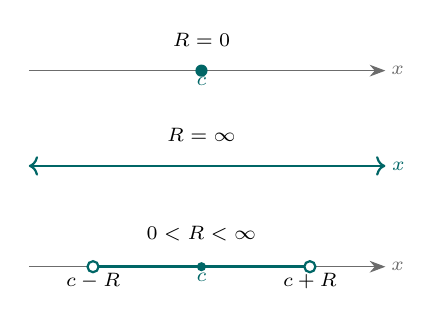
\begin{tikzpicture}[x=1.02cm,y=1cm]
                \draw[sumbu] (-2.15,2.76) -- (2.29,2.76) node[right,label grafik] {$x$};
                \fill[teal!80!black] (0,2.76) circle (2.2pt)
                    node[below,label grafik] {$c$};
                \node[above,label grafik] at (0,2.99) {$R=0$};
                \draw[pembanding,<->] (-2.15,1.55) -- (2.29,1.55)
                    node[right,label grafik] {$x$};
                \node[above,label grafik] at (0,1.78) {$R=\infty$};
                \draw[sumbu] (-2.15,.27) -- (2.29,.27) node[right,label grafik] {$x$};
                \draw[pembanding,very thick] (-1.35,.27) -- (1.35,.27);
                \foreach \posisi/\teks in {-1.35/{c-R},1.35/{c+R}} {
                    \filldraw[fill=white,draw=teal!80!black,thick]
                        (\posisi,.27) circle (2pt)
                        node[below,label grafik] {$\teks$};
                }
                \fill[teal!80!black] (0,.27) circle (1.65pt)
                    node[below,label grafik] {$c$};
                \node[above,label grafik] at (0,.52) {$0<R<\infty$};
            \end{tikzpicture}\par
            \small Tanda terbuka pada $c\pm R$ menandai titik yang perlu diuji.
        \end{column}
    \end{columns}
\end{frame}

\begin{frame}{\insertsection}
    \framesubtitle{Faktorial dapat membuat $R$ takhingga atau nol}
    \begin{columns}[T,onlytextwidth]
        \begin{column}{.48\textwidth}
            \begin{contoh}
                Tentukan $R$ untuk $\displaystyle\sum_{n=0}^\infty \frac{x^n}{n!}$.
            \end{contoh}
            \onslide<2->{Untuk $x\ne0$, rasio nilai mutlaknya
            \[
                \frac{|x|}{n+1}\to0
            \]
            bagi setiap $x$ tetap. Di $x=0$, deret bernilai $1$.
            Jadi $R=\infty$ dan selang konvergensinya $\R$.}
        \end{column}
        \begin{column}{.48\textwidth}
            \begin{contoh}
                Tentukan $R$ untuk $\displaystyle\sum_{n=0}^\infty n!x^n$.
            \end{contoh}
            \onslide<3->{Untuk $x\ne0$, rasio nilai mutlaknya
            \[
                (n+1)|x|\to\infty.
            \]
            Deret hanya konvergen di $x=0$, sehingga $R=0$.
            Di pusat, periksa deret langsung karena suku-suku
            berderajat positif sudah nol.}
        \end{column}
    \end{columns}
\end{frame}

\begin{frame}{\insertsection}
    \framesubtitle{Uji rasio memberi bagian dalam, lalu periksa kedua ujung}
    \begin{columns}[c,onlytextwidth]
        \begin{column}{.5\textwidth}
            \begin{contoh}
                Tentukan jari-jari dan selang konvergensi
                $\displaystyle\sum_{n=1}^\infty\frac{(x-2)^n}{3^n n}$.
            \end{contoh}
            \onslide<2->{Untuk $x\ne2$, rasio mutlaknya menuju
            \[
                \frac{|x-2|}{3}\lim_{n\to\infty}\frac{n}{n+1}
                =\frac{|x-2|}{3}.
            \]
            Maka $R=3$, dengan bagian dalam $-1<x<5$.
            Di pusat $x=2$, deret bernilai $0$.}
        \end{column}
        \begin{column}{.46\textwidth}
            \onslide<3->{%
                \begin{block}{Substitusikan kedua titik ujung}
                    Pada $x=-1$ diperoleh $\sum(-1)^n/n$,
                    yang konvergen bersyarat.
                    Pada $x=5$ diperoleh $\sum 1/n$, yang divergen.
                    Jadi selang konvergensinya $[-1,5)$.
                \end{block}
                \centering
                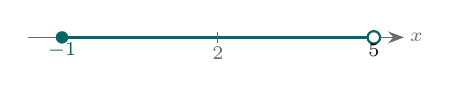
\begin{tikzpicture}[x=.66cm]
                    \draw[sumbu] (-1.65,0) -- (5.58,0)
                        node[right,label grafik] {$x$};
                    \draw[pembanding,very thick] (-1,0) -- (5,0);
                    \fill[teal!80!black] (-1,0) circle (2.25pt)
                        node[below,label grafik] {$-1$};
                    \filldraw[fill=white,draw=teal!80!black,thick] (5,0) circle (2.25pt)
                        node[below,label grafik] {$5$};
                    \draw[gray!80!black] (2,-.07) -- (2,.07)
                        node[below=.12cm,label grafik] {$2$};
                \end{tikzpicture}\par
            }
        \end{column}
    \end{columns}
\end{frame}

\begin{frame}{\insertsection}
    \framesubtitle{Polinomial Maclaurin mencocokkan nilai dan turunan di nol}
    \begin{columns}[c,onlytextwidth]
        \begin{column}{.51\textwidth}
            \begin{definisi}[Polinomial Maclaurin]
                Jika $f$ dapat diturunkan sampai orde $N$ di $0$,
                polinomial Maclaurin orde $N$ ialah
                \[
                    P_N(x)=\sum_{k=0}^N\frac{f^{(k)}(0)}{k!}\,x^k.
                \]
                Di sini $f^{(0)}=f$ dan $0!=1$.
            \end{definisi}
            Polinomialnya memiliki nilai dan turunan orde
            $1$ sampai $N$ yang sama dengan $f$ di $x=0$.
        \end{column}
        \begin{column}{.45\textwidth}
            \begin{block}{Dari turunan ke koefisien}
                Jika $P_N(x)=c_0+c_1x+\cdots+c_Nx^N$,
                maka $P_N^{(k)}(0)=k!\,c_k$.
                Mencocokkan dengan $f^{(k)}(0)$ menentukan
                tepat satu nilai untuk setiap $c_k$.
            \end{block}
            \begin{contoh}
                Untuk $f(x)=e^x$, semua $f^{(k)}(0)=1$.
                Maka $P_0=1$, $P_1=1+x$, dan
                $P_2=1+x+x^2/2$.
            \end{contoh}
        \end{column}
    \end{columns}
\end{frame}

\begin{frame}{\insertsection}
    \framesubtitle{Polinomial eksponensial berimpit makin dekat di sekitar pusat}
    \begin{columns}[c,onlytextwidth]
        \begin{column}{.51\textwidth}
            \begin{contoh}
                Hampiri $e^{-0{,}4}$ dengan polinomial Maclaurin orde $3$.
            \end{contoh}
            \onslide<2->{Tambahkan suku kubik pada $P_2$.
            \[
                P_3(x)=1+x+\frac{x^2}{2}+\frac{x^3}{6}.
            \]
            Dengan $x=-0{,}4$, diperoleh
            $P_3(-0{,}4)\approx0{,}66933$.}
            \onslide<3->{Nilai $e^{-0{,}4}\approx0{,}67032$,
            sehingga selisihnya sekitar $0{,}00099$.
            Di $0$, bahkan nilai dan tiga turunan pertamanya sama.}
        \end{column}
        \begin{column}{.45\textwidth}
            \centering
            \begin{tikzpicture}
                \begin{axis}[bidang,width=5.85cm,height=3.92cm,
                    xmin=-1.87,xmax=1.88,ymin=-.8,ymax=5.92,
                    xlabel={$x$},ylabel={$y$},xtick={-1,1},ytick={1,3,5}]
                    \addplot[kurva,domain=-1.78:1.75] {exp(x)};
                    \addplot[gray!85!black,dashed,thick,domain=-1.78:1.75] {1+x};
                    \addplot[pembanding,dashdotted,domain=-1.78:1.75] {1+x+x^2/2};
                    \only<2->{\addplot[magenta,densely dashed,thick,domain=-1.78:1.75]
                        {1+x+x^2/2+x^3/6};}
                    \addplot[suku] coordinates {(0,1)};
                \end{axis}
            \end{tikzpicture}\par
            \small
            \textcolor{HIMAtua}{$e^x$}\quad
            \textcolor{gray!85!black}{$P_1$}\quad
            \textcolor{teal!80!black}{$P_2$}\quad
            \onslide<2->{\textcolor{magenta}{$P_3$}}
        \end{column}
    \end{columns}
\end{frame}

\begin{frame}{\insertsection}
    \framesubtitle{Pusat Taylor dapat dipilih di sekitar nilai yang akan dihampiri}
    \begin{columns}[c,onlytextwidth]
        \begin{column}{.52\textwidth}
            \begin{definisi}[Polinomial Taylor]
                Jika $f$ dapat diturunkan sampai orde $N$ di $a$,
                polinomial Taylor orde $N$ terhadap pusat $a$ ialah
                \[
                    P_N(x)=\sum_{k=0}^N
                        \frac{f^{(k)}(a)}{k!}(x-a)^k.
                \]
            \end{definisi}
            Yang dicocokkan adalah $P_N^{(k)}(a)=f^{(k)}(a)$
            untuk $0\le k\le N$. Memilih $a=0$ memberi Maclaurin.
        \end{column}
        \begin{column}{.44\textwidth}
            \begin{block}{Baca jarak dari pusat}
                Pangkat $(x-a)^k$ kecil di sekitar $a$.
                Contohnya, untuk $f(x)=\ln x$ dan $a=3$,
                suku konstan adalah $\ln 3$, lalu suku linear
                adalah $\tfrac13(x-3)$.
            \end{block}
            \onslide<2->{Polinomial orde $1$ ini adalah garis singgung
            $\ln x$ di $x=3$. Orde berikutnya mengikuti
            turunan yang lebih tinggi di titik itu.}
        \end{column}
    \end{columns}
\end{frame}

\begin{frame}{\insertsection}
    \framesubtitle{Koefisien di sekitar $x=3$ berasal dari turunan $\ln x$ di $3$}
    \begin{columns}[c,onlytextwidth]
        \begin{column}{.52\textwidth}
            \begin{contoh}
                Bentuk $P_3$ untuk $f(x)=\ln x$ dengan pusat $3$.
            \end{contoh}
            \onslide<2->{%
                \[
                    f'(3)=\frac13,\quad f''(3)=-\frac19,\quad
                    f'''(3)=\frac2{27}.
                \]
                Bagi dengan $1!$, $2!$, dan $3!$.
            }
            \onslide<3->{%
                \[
                    \begin{aligned}
                        P_3(x)=\ln3+\frac{x-3}{3}
                        &-\frac{(x-3)^2}{18}\\
                        &+\frac{(x-3)^3}{81}.
                    \end{aligned}
                \]
            }
        \end{column}
        \begin{column}{.44\textwidth}
            \centering
            \begin{tikzpicture}
                \begin{axis}[bidang,width=5.8cm,height=3.9cm,
                    xmin=.39,xmax=5.55,ymin=-.82,ymax=2.16,
                    xlabel={$x$},ylabel={$y$},xtick={1,3,5},ytick={1,2}]
                    \addplot[kurva,domain=.55:5.35] {ln(x)};
                    \addplot[gray!85!black,thick,dashed,domain=.55:5.35] {ln(3)+(x-3)/3};
                    \only<2->{\addplot[pembanding,dashdotted,domain=.55:5.35]
                        {ln(3)+(x-3)/3-(x-3)^2/18};}
                    \only<3->{\addplot[magenta,thick,densely dashed,domain=.55:5.35]
                        {ln(3)+(x-3)/3-(x-3)^2/18+(x-3)^3/81};}
                    \draw[bantu] (axis cs:3,0) -- (axis cs:3,1.098612);
                    \addplot[suku] coordinates {(3,1.098612)};
                \end{axis}
            \end{tikzpicture}\par
            \small
            \textcolor{HIMAtua}{$\ln x$}\quad
            \textcolor{gray!85!black}{$P_1$}\quad
            \onslide<2->{\textcolor{teal!80!black}{$P_2$}}\quad
            \onslide<3->{\textcolor{magenta}{$P_3$}}
        \end{column}
    \end{columns}
\end{frame}

\begin{frame}{\insertsection}
    \framesubtitle{Polinomial Taylor adalah jumlah parsial dari deret Taylor}
    \begin{columns}[c,onlytextwidth]
        \begin{column}{.52\textwidth}
            \begin{definisi}[Deret Taylor dan Maclaurin]
                Jika $f$ memiliki turunan semua orde di $a$,
                deret Taylor berpusat di $a$ adalah
                \[
                    \sum_{k=0}^\infty\frac{f^{(k)}(a)}{k!}(x-a)^k.
                \]
                Untuk $a=0$, deret ini disebut deret Maclaurin.
            \end{definisi}
            Jumlah dari indeks $0$ sampai $N$ adalah $P_N(x)$.
            Deret mewakili $f(x)$ di titik yang memenuhi
            $f(x)-P_N(x)\to0$.
        \end{column}
        \begin{column}{.44\textwidth}
            \begin{contoh}
                Karena semua turunan $e^x$ di $0$ bernilai $1$,
                deret Maclaurin-nya ialah
                \[
                    \sum_{k=0}^\infty \frac{x^k}{k!}
                    =1+x+\frac{x^2}{2!}+\frac{x^3}{3!}+\cdots.
                \]
            \end{contoh}
            \onslide<2->{Uji rasio memberi $R=\infty$.
            Batas sisa memungkinkan kita menunjukkan
            bahwa jumlah tersebut benar-benar sama dengan $e^x$.}
        \end{column}
    \end{columns}
\end{frame}

\begin{frame}{\insertsection}
    \framesubtitle{Sisa Taylor mengukur kapan hampiran menjadi identitas}
    \begin{columns}[c,onlytextwidth]
        \begin{column}{.51\textwidth}
            \begin{block}{Batas sisa Lagrange}
                Jika turunan sampai orde $N+1$ kontinu pada
                selang antara $a$ dan $x$ dan
                $|f^{(N+1)}(t)|\le M$ di selang itu, maka
                \[
                    |f(x)-P_N(x)|
                    \le \frac{M|x-a|^{N+1}}{(N+1)!}.
                \]
            \end{block}
            Batas berasal dari rumus sisa
            $f^{(N+1)}(\xi)(x-a)^{N+1}/(N+1)!$
            untuk suatu $\xi$ di antara $a$ dan $x$.
        \end{column}
        \begin{column}{.45\textwidth}
            \begin{contoh}
                Untuk $e^x$ berpusat di $0$, dapat dipakai
                $M=e^{|x|}$ pada selang antara $0$ dan $x$.
            \end{contoh}
            \onslide<2->{Untuk $x$ tetap, $M$ bebas dari $N$.
            Rasio batas galat berturut-turut ialah $|x|/(N+2)\to0$,
            sehingga batas galat menuju nol.
            \[
                e^x=\sum_{k=0}^\infty\frac{x^k}{k!}
                \quad(x\in\R).
            \]}
        \end{column}
    \end{columns}
\end{frame}

\begin{frame}{\insertsection}
    \framesubtitle{Siklus empat turunan menyisakan pangkat ganjil atau genap}
    \begin{columns}[T,onlytextwidth]
        \begin{column}{.48\textwidth}
            \begin{contoh}[Sinus]
                Urutan nilai turunan di $0$ adalah
                $0,1,0,-1$, lalu berulang.
            \end{contoh}
            \onslide<2->{Suku yang tersisa berpangkat ganjil.
            \[
                \sin x=\sum_{k=0}^\infty
                    \frac{(-1)^k x^{2k+1}}{(2k+1)!}
                = x-\frac{x^3}{3!}+\frac{x^5}{5!}-\cdots.
            \]}
        \end{column}
        \begin{column}{.48\textwidth}
            \begin{contoh}[Kosinus]
                Urutan nilai turunan di $0$ adalah
                $1,0,-1,0$, lalu berulang.
            \end{contoh}
            \onslide<3->{Suku yang tersisa berpangkat genap.
            \[
                \cos x=\sum_{k=0}^\infty
                    \frac{(-1)^k x^{2k}}{(2k)!}
                =1-\frac{x^2}{2!}+\frac{x^4}{4!}-\cdots.
            \]}
        \end{column}
    \end{columns}
    \onslide<4->{Kedua identitas berlaku untuk setiap $x\in\R$.
    Semua turunan sinus dan kosinus dibatasi oleh $1$ dalam nilai mutlak,
    sehingga batas sisa Taylor menuju nol.
    Gunakan sudut dalam radian.}
\end{frame}

\begin{frame}{\insertsection}
    \framesubtitle{Bentuk grafik mengikuti suku yang masih dipertahankan}
    \begin{columns}[c,onlytextwidth]
        \begin{column}{.47\textwidth}
            \centering
            \begin{tikzpicture}
                \begin{axis}[bidang,width=6.15cm,height=3.89cm,
                    xmin=-3.32,xmax=3.39,ymin=-2.25,ymax=2.25,
                    xlabel={$x$},ylabel={$y$},xtick={-3,3},ytick={-1,1}]
                    \addplot[kurva,domain=-3.22:3.22] {sin(deg(x))};
                    \addplot[pembanding,dashed,domain=-3.22:3.22] {x-x^3/6};
                    \only<2->{\addplot[magenta,thick,dashdotted,domain=-3.22:3.22]
                        {x-x^3/6+x^5/120-x^7/5040};}
                \end{axis}
            \end{tikzpicture}\par
            \small
            \textcolor{HIMAtua}{$\sin x$}\quad
            \textcolor{teal!80!black}{$P_3$}\quad
            \onslide<2->{\textcolor{magenta}{$P_7$}}
        \end{column}
        \begin{column}{.47\textwidth}
            \centering
            \begin{tikzpicture}
                \begin{axis}[bidang,width=6.15cm,height=3.89cm,
                    xmin=-3.32,xmax=3.39,ymin=-2.25,ymax=1.45,
                    xlabel={$x$},ylabel={$y$},xtick={-3,3},ytick={-1,1}]
                    \addplot[kurva,domain=-3.22:3.22] {cos(deg(x))};
                    \addplot[pembanding,dashed,domain=-3.22:3.22] {1-x^2/2};
                    \only<2->{\addplot[magenta,thick,dashdotted,domain=-3.22:3.22]
                        {1-x^2/2+x^4/24-x^6/720};}
                \end{axis}
            \end{tikzpicture}\par
            \small
            \textcolor{HIMAtua}{$\cos x$}\quad
            \textcolor{teal!80!black}{$P_2$}\quad
            \onslide<2->{\textcolor{magenta}{$P_6$}}
        \end{column}
    \end{columns}
    \onslide<2->{Koefisien yang nol juga berguna. Untuk sinus,
    $P_4=P_3$ karena turunan orde $4$ di $0$ nol.
    Untuk kosinus, $P_3=P_2$ dengan alasan serupa.}
\end{frame}

\begin{frame}{\insertsection}
    \framesubtitle{Fungsi resiprokal di sekitar pusat bukan nol}
    \begin{columns}[T,onlytextwidth]
        \begin{column}{.49\textwidth}
            \begin{contoh}
                Dapatkan deret Taylor $f(x)=1/x$ berpusat di $2$.
            \end{contoh}
            \onslide<2->{Pola turunan memberi
            $f^{(k)}(x)=(-1)^k k!/x^{k+1}$. Maka
            \[
                \sum_{k=0}^\infty\frac{(-1)^k(x-2)^k}{2^{k+1}}.
            \]
            Rasionya $r=-(x-2)/2$.}
        \end{column}
        \begin{column}{.47\textwidth}
            \onslide<3->{%
                \begin{block}{Uji dengan bentuk geometrik}
                    \[
                        \frac1x=\frac{1/2}{1+(x-2)/2}.
                    \]
                    Dengan $|r|<1$, jumlah deret di kiri
                    sama dengan fungsi ini. Jadi $R=2$.
                \end{block}
                Pada kedua ujung $x=0$ dan $x=4$, nilai mutlak
                suku tetap $1/2$. Selang konvergensinya $(0,4)$.
            }
        \end{column}
    \end{columns}
\end{frame}

\begin{frame}{\insertsection}
    \framesubtitle{Substitusi mewarisi syarat konvergensi deret asal}
    \begin{columns}[T,onlytextwidth]
        \begin{column}{.47\textwidth}
            \begin{contoh}
                Bentuk deret Maclaurin untuk $1/(1-3x^2)$.
            \end{contoh}
            \onslide<2->{Dari $\frac1{1-u}=\sum_{k=0}^\infty u^k$
            untuk $|u|<1$, pakai $u=3x^2$.
            \[
                \frac1{1-3x^2}=\sum_{k=0}^\infty 3^k x^{2k}
                \quad\left(|x|<\frac1{\sqrt3}\right).
            \]
            Pada $x=\pm1/\sqrt3$, setiap suku bernilai $1$.}
        \end{column}
        \begin{column}{.49\textwidth}
            \begin{contoh}
                Bentuk deret untuk $\cosh x$ dan $\sinh x$.
            \end{contoh}
            \onslide<3->{Dari deret $e^x$ dan substitusi $-x$,
            \[
                \begin{aligned}
                    \cosh x&=\frac{e^x+e^{-x}}2
                         =\sum_{k=0}^\infty\frac{x^{2k}}{(2k)!},\\
                    \sinh x&=\frac{e^x-e^{-x}}2
                         =\sum_{k=0}^\infty\frac{x^{2k+1}}{(2k+1)!}.
                \end{aligned}
            \]
            Keduanya berlaku untuk semua $x$ real.}
        \end{column}
    \end{columns}
\end{frame}

\begin{frame}{\insertsection}
    \framesubtitle{Koefisien binomial tetap terdefinisi untuk pangkat real}
    \begin{columns}[c,onlytextwidth]
        \begin{column}{.52\textwidth}
            \begin{block}{Deret binomial}
                Untuk $m\in\R$ dan $|x|<1$,
                \[
                    (1+x)^m=\sum_{k=0}^\infty\binom{m}{k}x^k,\qquad
                    \binom{m}{0}=1,
                \]
                dengan $\displaystyle\binom{m}{k}
                =\frac{m(m-1)\cdots(m-k+1)}{k!}$ untuk $k\ge1$.
            \end{block}
            Pembilang adalah pola turunan $(1+x)^m$ di nol.
            Bila $m$ bulat tak negatif, deret berhenti
            dan menjadi polinomial untuk semua $x$.
        \end{column}
        \begin{column}{.44\textwidth}
            \begin{contoh}
                Untuk $m=\tfrac12$ dan $|x|<1$, diperoleh
                \[
                    \sqrt{1+x}=1+\frac x2-\frac{x^2}{8}
                        +\frac{x^3}{16}-\cdots.
                \]
            \end{contoh}
            \onslide<2->{Jika deret tidak berhenti, rasio koefisien
            mutlaknya menuju $1$ karena
            $\left|\binom{m}{k+1}/\binom{m}{k}\right|
            =|m-k|/(k+1)$. Maka $R=1$.}
        \end{column}
    \end{columns}
\end{frame}

\begin{frame}{\insertsection}
    \framesubtitle{Pada deret binomial takhingga, status titik ujung bergantung pada pangkat}
    \begin{columns}[c,onlytextwidth]
        \begin{column}{.52\textwidth}
            \begin{block}{Konvergensi di $x=\pm1$}
                Untuk deret binomial yang tidak berhenti,
                \[
                    \begin{array}{c|c|c}
                        m & x=-1 & x=1\\ \hline
                        m>0 & \text{mutlak} & \text{mutlak}\\
                        -1<m<0 & \text{divergen} & \text{bersyarat}\\
                        m\le-1 & \text{divergen} & \text{divergen}
                    \end{array}
                \]
                Rasio mutlak suku di kedua titik menuju $1$.
            \end{block}
            Perubahan dari $x=1$ ke $x=-1$ mengalikan suku
            ke-$k$ dengan $(-1)^k$. Besar sukunya tetap,
            tetapi pola tandanya berubah.
        \end{column}
        \begin{column}{.44\textwidth}
            \begin{contoh}
                Ambil $m=-\tfrac12$. Tuliskan
                $\binom{-1/2}{k}=(-1)^k b_k$.
                Maka $b_{k+1}/b_k=(k+\tfrac12)/(k+1)$.
            \end{contoh}
            \onslide<2->{Di $x=1$, deretnya berganti tanda
            dan konvergen bersyarat. Di $x=-1$, faktor $(-1)^k$
            menghilangkan tanda berselang. Deret positif
            tersebut divergen sesuai tabel.}
        \end{column}
    \end{columns}
\end{frame}

\begin{frame}{\insertsection}
    \framesubtitle{Latihan jari-jari, titik ujung, dan pemilihan pusat}
    \begin{columns}[T,onlytextwidth]
        \begin{column}{.47\textwidth}
            \begin{latihan}
                \begin{enumerate}
                    \item Tentukan selang konvergensi
                        $\sum_{n=1}^\infty (x+1)^n/(2^n n^2)$.
                    \item Bentuk polinomial Taylor orde $3$
                        dari $\ln x$ berpusat di $1$.
                    \item Tuliskan tiga suku awal deret Maclaurin
                        untuk $e^{-x^2}$ dan jari-jarinya.
                \end{enumerate}
            \end{latihan}
        \end{column}
        \begin{column}{.49\textwidth}
            \onslide<2->{%
                \begin{block}{Cek jawaban}
                    \begin{enumerate}
                        \item $R=2$. Pada $-3$ dan $1$,
                            deret nilai mutlaknya $\sum 1/n^2$.
                            Jadi selangnya $[-3,1]$.
                        \item $(x-1)-\tfrac12(x-1)^2+\tfrac13(x-1)^3$.
                        \item $1-x^2+x^4/2+\cdots$ dari substitusi
                            $-x^2$ pada $e^x$, dengan $R=\infty$.
                    \end{enumerate}
                \end{block}
            }
        \end{column}
    \end{columns}
\end{frame}

% Kalkulus 2 Bab 6.pdf, subbab 6.5.
\section{Diferensiasi dan Integrasi Deret Pangkat}

\begin{frame}{\insertsection}
    \framesubtitle{Representasi berarti jumlah deret sama dengan fungsi pada selangnya}
    \begin{columns}[c,onlytextwidth]
        \begin{column}{.53\textwidth}
            \begin{definisi}[Representasi deret pangkat]
                Deret $\sum_{k=0}^{\infty}c_k(x-a)^k$
                merepresentasikan $f$ pada selang $I$ jika
                untuk setiap $x\in I$ deret konvergen dan
                jumlahnya sama dengan $f(x)$.
            \end{definisi}
            Nilai $f$ pada suatu titik diperoleh sebagai
            limit polinomial jumlah parsial di titik itu.
        \end{column}
        \begin{column}{.43\textwidth}
            \begin{contoh}
                Rumus geometrik memberi
                \[
                    \frac1{1-x}=1+x+x^2+x^3+\cdots
                    \quad (|x|<1).
                \]
            \end{contoh}
            \onslide<2->{Pada $x=-1/2$, deret bernilai $2/3$.
            Pada $x=2$, fungsi rasionalnya bernilai $-1$
            dan deret $1+2+4+\cdots$ divergen.
            Selang representasi perlu dicantumkan.}
        \end{column}
    \end{columns}
\end{frame}

\begin{frame}{\insertsection}
    \framesubtitle{Diferensiasi suku per suku mempertahankan jari-jari}
    \begin{columns}[c,onlytextwidth]
        \begin{column}{.54\textwidth}
            \begin{teorema}[Diferensiasi deret pangkat]
                Misalkan $f(x)=\sum_{k=0}^\infty c_k(x-a)^k$
                pada bagian dalam jari-jari $R>0$.
                Deret turunannya juga mempunyai jari-jari $R$,
                dan untuk $|x-a|<R$,
                \[
                    f'(x)=\sum_{k=1}^\infty k c_k(x-a)^{k-1}.
                \]
            \end{teorema}
            Suku konstan hilang. Di titik ujung, uji deret hasil
            diferensiasi secara terpisah.
        \end{column}
        \begin{column}{.42\textwidth}
            \begin{contoh}[Turunan sinus]
                Diferensiasi suku ke-$k$ deret $\sin x$ memberi
                \[
                    \frac{d}{dx}\left[\frac{(-1)^kx^{2k+1}}{(2k+1)!}\right]
                    =\frac{(-1)^k x^{2k}}{(2k)!}.
                \]
                Jumlahnya adalah deret untuk $\cos x$,
                berlaku di seluruh $\R$.
            \end{contoh}
        \end{column}
    \end{columns}
\end{frame}

\begin{frame}{\insertsection}
    \framesubtitle{Indeks dapat digeser agar deret turunan mulai dari pangkat nol}
    \begin{columns}[T,onlytextwidth]
        \begin{column}{.47\textwidth}
            \begin{contoh}[Eksponensial]
                Turunkan deret Maclaurin $e^x$.
            \end{contoh}
            \onslide<2->{%
                \[
                    \frac{d}{dx}\sum_{k=0}^\infty\frac{x^k}{k!}
                    =\sum_{k=1}^\infty\frac{x^{k-1}}{(k-1)!}.
                \]
                Dengan $j=k-1$, hasilnya menjadi
                $\sum_{j=0}^\infty x^j/j!=e^x$.}
        \end{column}
        \begin{column}{.49\textwidth}
            \begin{contoh}[Geometrik]
                Turunkan $1/(1-x)=\sum_{k=0}^\infty x^k$.
            \end{contoh}
            \onslide<3->{Pada $|x|<1$,
            \[
                \frac1{(1-x)^2}
                    =\sum_{k=1}^\infty kx^{k-1}
                    =\sum_{j=0}^\infty (j+1)x^j.
            \]
            Bentuk ini membantu menjumlahkan deret yang
            sukunya mempunyai faktor $k$.}
        \end{column}
    \end{columns}
\end{frame}

\begin{frame}{\insertsection}
    \framesubtitle{Integrasi suku per suku menambahkan satu konstanta untuk seluruh deret}
    \begin{columns}[c,onlytextwidth]
        \begin{column}{.52\textwidth}
            \begin{teorema}[Integrasi deret pangkat]
                Misalkan $f(x)=\sum_{k=0}^\infty c_k(x-a)^k$
                untuk $|x-a|<R$ dengan $R>0$.
                Fungsi $f$ kontinu pada selang ini dan
                \[
                    \int f(x)\,dx=C+
                    \sum_{k=0}^\infty\frac{c_k}{k+1}(x-a)^{k+1}.
                \]
                Deret antiturunannya juga berjari-jari $R$.
            \end{teorema}
            Untuk menentukan $C$, gunakan nilai antiturunan
            di $x=a$. Semua suku dalam sigma bernilai nol di sana.
        \end{column}
        \begin{column}{.44\textwidth}
            \begin{block}{Integral tertentu}
                Jika $\alpha,\beta$ berada di $(a-R,a+R)$,
                \[
                    \int_\alpha^\beta f(x)\,dx
                     =\sum_{k=0}^\infty\frac{c_k}{k+1}
                       \left[(x-a)^{k+1}\right]_\alpha^\beta .
                \]
                Deret hasil evaluasi batas konvergen mutlak.
            \end{block}
            Untuk $\alpha=a$, hanya substitusi batas atas
            yang menyumbang pada deret.
        \end{column}
    \end{columns}
\end{frame}

\begin{frame}{\insertsection}
    \framesubtitle{Deret antiturunan diperoleh dengan menaikkan pangkat}
    \begin{columns}[T,onlytextwidth]
        \begin{column}{.46\textwidth}
            \begin{contoh}[Integrasi kosinus]
                Integralkan deret Maclaurin $\cos x$.
            \end{contoh}
            \onslide<2->{%
                \[
                    \int\cos x\,dx=C+
                    \sum_{k=0}^\infty
                       \frac{(-1)^k x^{2k+1}}{(2k+1)(2k)!}.
                \]
                Karena $(2k+1)(2k)!=(2k+1)!$,
                jumlahnya adalah $\sin x+C$ untuk semua $x$.}
        \end{column}
        \begin{column}{.5\textwidth}
            \begin{contoh}[Logaritma]
                Mulai dari $1/(1+t)=\sum_{k=0}^\infty(-t)^k$.
                Integralkan dari $0$ ke $x$.
            \end{contoh}
            \onslide<3->{Untuk $|x|<1$,
            \[
                \ln(1+x)=\sum_{k=0}^\infty
                    \frac{(-1)^k x^{k+1}}{k+1}.
            \]
            Suku awalnya $x-x^2/2+x^3/3-\cdots$.
            Mendiferensiasikannya pada $|x|<1$ memberi
            kembali deret untuk $1/(1+x)$.}
        \end{column}
    \end{columns}
\end{frame}

\begin{frame}{\insertsection}
    \framesubtitle{Integrasi polinomial memberi hampiran untuk luas di bawah kurva}
    \begin{columns}[c,onlytextwidth]
        \begin{column}{.53\textwidth}
            \begin{contoh}
                Bentuk deret yang menjumlah ke
                $\displaystyle I=\int_0^{1/2} e^{-x^2}\,dx$.
            \end{contoh}
            \onslide<2->{Substitusi $-x^2$ pada deret eksponensial
            memberi $\sum_{k=0}^\infty(-1)^k x^{2k}/k!$.
            Jari-jarinya takhingga, sehingga kedua batas
            integral berada di bagian dalam.}
            \onslide<3->{Integrasikan suku per suku.
            \[
                I=\sum_{k=0}^\infty
                  \frac{(-1)^k(1/2)^{2k+1}}{(2k+1)k!}.
            \]}
        \end{column}
        \begin{column}{.43\textwidth}
            \centering
            \begin{tikzpicture}
                \begin{axis}[bidang,width=5.7cm,height=3.95cm,
                    xmin=-.08,xmax=1.12,ymin=0,ymax=1.22,
                    xlabel={$x$},ylabel={$y$},xtick={.5,1},
                    xticklabels={$1/2$,$1$},ytick={1}]
                    \addplot[draw=none,fill=HIMAmuda!37,domain=0:.5]
                        {exp(-x^2)} \closedcycle;
                    \addplot[kurva,domain=0:1.05] {exp(-x^2)};
                    \draw[bantu] (axis cs:.5,0) -- (axis cs:.5,.778801);
                    \node[HIMAtua,label grafik] at (axis cs:.27,.43) {$I$};
                    \node[HIMAtua,label grafik] at (axis cs:.75,.85) {$e^{-x^2}$};
                \end{axis}
            \end{tikzpicture}
        \end{column}
    \end{columns}
\end{frame}

\begin{frame}{\insertsection}
    \framesubtitle{Suku berikutnya membatasi galat integral dari deret berselang}
    \begin{columns}[c,onlytextwidth]
        \begin{column}{.49\textwidth}
            \begin{contoh}
                Hampiri $I=\int_0^{1/2}e^{-x^2}\,dx$
                dengan tiga suku pertama.
            \end{contoh}
            \onslide<2->{Ambil suku dengan $k=0,1,2$.
            \[
                I_3=\frac12-\frac1{24}+\frac1{320}
                    \approx0{,}46146.
            \]}
        \end{column}
        \begin{column}{.47\textwidth}
            \onslide<3->{%
                \begin{block}{Batas galat}
                    Tanda suku bergantian dan nilai mutlaknya
                    turun. Rasionya
                    $\frac{2k+1}{4(k+1)(2k+3)}<1$.
                    Suku berikutnya memiliki besar
                    \[
                        \frac{(1/2)^7}{7\cdot3!}=\frac1{5376}.
                    \]
                    Dari batas sisa deret berganti tanda,
                    $I_3-1/5376\le I\le I_3$.
                \end{block}
            }
        \end{column}
    \end{columns}
\end{frame}

\begin{frame}{\insertsection}
    \framesubtitle{Turunan berulang di pusat menentukan setiap koefisien}
    \begin{columns}[c,onlytextwidth]
        \begin{column}{.53\textwidth}
            \begin{teorema}[Ketunggalan representasi deret pangkat]
                Jika $f(x)=\sum_{k=0}^\infty c_k(x-a)^k$
                pada suatu selang terbuka yang memuat $a$,
                maka $c_k=f^{(k)}(a)/k!$. Deret tersebut
                adalah deret Taylor $f$ berpusat di $a$.
            \end{teorema}
            Setiap kali diturunkan, pangkat turun satu.
            Setelah $k$ kali, evaluasi di $a$ hanya menyisakan $k!\,c_k$.
        \end{column}
        \begin{column}{.43\textwidth}
            \begin{block}{Beberapa koefisien pertama}
                \[
                    f(a)=c_0,\quad f'(a)=c_1,\quad
                    f''(a)=2!\,c_2.
                \]
                Cara ini menjelaskan mengapa substitusi,
                integrasi, atau diferensiasi yang memberi
                representasi di sekitar $a$ menghasilkan
                koefisien Taylor yang sama.
            \end{block}
        \end{column}
    \end{columns}
\end{frame}

\begin{frame}{\insertsection}
    \framesubtitle{Arctan diperoleh dengan mengintegralkan deret geometrik}
    \begin{columns}[c,onlytextwidth]
        \begin{column}{.51\textwidth}
            \begin{contoh}
                Dapatkan deret Maclaurin untuk $\arctan x$.
            \end{contoh}
            \onslide<2->{Substitusi $-t^2$ pada deret geometrik.
            \[
                \frac1{1+t^2}=\sum_{k=0}^\infty (-1)^k t^{2k}
                \quad(|t|<1).
            \]
            Karena $\arctan 0=0$, gunakan
            $\arctan x=\int_0^x (1+t^2)^{-1}\,dt$.}
        \end{column}
        \begin{column}{.45\textwidth}
            \onslide<3->{Integrasi memberi
            \[
                \arctan x=\sum_{k=0}^\infty
                  \frac{(-1)^k x^{2k+1}}{2k+1}
                \quad(|x|<1).
            \]
            Suku awalnya $x-x^3/3+x^5/5-\cdots$.
            Pusatnya $0$, sehingga representasi ini adalah
            deret Maclaurin $\arctan x$.}
        \end{column}
    \end{columns}
\end{frame}

\begin{frame}{\insertsection}
    \framesubtitle{Integrasi dapat menambahkan titik ujung pada selang konvergensi}
    Untuk $j=1,2$ dan $0\le t\le1$, gunakan jumlah geometrik berhingga
    \[
        \frac1{1+t^j}=\sum_{k=0}^N(-t^j)^k+\frac{(-t^j)^{N+1}}{1+t^j}.
    \]
    \onslide<2->{Nilai mutlak integral suku sisa dari $0$ ke $1$ dibatasi oleh
    $\int_0^1 t^{j(N+1)}\,dt=1/[j(N+1)+1]\to0$.}
    \begin{columns}[T,onlytextwidth]
        \begin{column}{.47\textwidth}
            \onslide<3->{%
                \begin{block}{Logaritma}
                    Untuk $j=1$, jumlah di $x=1$ adalah $\ln2$.
                    Di $x=-1$, suku-sukunya $-1/(k+1)$ dan
                    deret divergen. Selangnya $(-1,1]$.
                \end{block}
            }
        \end{column}
        \begin{column}{.49\textwidth}
            \onslide<4->{%
                \begin{block}{Arctan}
                    Untuk $j=2$, jumlah di $x=1$ adalah $\pi/4$.
                    Karena deret dan fungsi sama-sama ganjil,
                    jumlah di $x=-1$ adalah $-\pi/4$.
                    Selangnya $[-1,1]$.
                \end{block}
            }
        \end{column}
    \end{columns}
\end{frame}

\begin{frame}{\insertsection}
    \framesubtitle{Perkalian deret mengikuti penjumlahan pangkat}
    \begin{columns}[c,onlytextwidth]
        \begin{column}{.51\textwidth}
            \begin{contoh}
                Dapatkan tiga suku tak nol pertama dari deret
                Maclaurin $e^{-2x^2}\arctan x$.
            \end{contoh}
            \onslide<2->{Untuk $|x|<1$, deret kedua faktor
            konvergen mutlak. Ambil suku yang dapat
            menghasilkan pangkat sampai $5$.
            \[
                \begin{aligned}
                    e^{-2x^2}&=1-2x^2+2x^4+\cdots,\\
                    \arctan x&=x-\frac{x^3}{3}+\frac{x^5}{5}-\cdots.
                \end{aligned}
            \]}
        \end{column}
        \begin{column}{.45\textwidth}
            \onslide<3->{%
                \begin{block}{Koefisien hasil kali}
                    \[
                        \begin{array}{c|l}
                            \text{Pangkat} & \text{Kontribusi}\\ \hline
                            1 & 1\\
                            3 & -1/3-2\\
                            5 & 1/5+2/3+2
                        \end{array}
                    \]
                \end{block}
                Jadi tiga suku yang diminta adalah
                \[
                    x-\frac73x^3+\frac{43}{15}x^5.
                \]
            }
        \end{column}
    \end{columns}
\end{frame}

\begin{frame}{\insertsection}
    \framesubtitle{Pembagian deret dapat dikerjakan dengan mencocokkan koefisien}
    \begin{columns}[c,onlytextwidth]
        \begin{column}{.52\textwidth}
            \begin{contoh}
                Dapatkan tiga suku tak nol pertama dari deret
                Maclaurin $\tan x$.
            \end{contoh}
            \onslide<2->{Di sekitar $0$, $\cos x\ne0$.
            Fungsi $\tan x$ ganjil, sehingga tulis
            $\tan x=b_1x+b_3x^3+b_5x^5+\cdots$.
            Gunakan $\tan x\cos x=\sin x$.
            \[
                \begin{aligned}
                    \cos x&=1-x^2/2+x^4/24-\cdots,\\
                    \sin x&=x-x^3/6+x^5/120-\cdots.
                \end{aligned}
            \]}
        \end{column}
        \begin{column}{.44\textwidth}
            \onslide<3->{%
                \begin{block}{Samakan pangkat yang sejenis}
                    \[
                        \begin{aligned}
                            b_1&=1,\\
                            b_3-b_1/2&=-1/6,\\
                            b_5-b_3/2+b_1/24&=1/120.
                        \end{aligned}
                    \]
                \end{block}
                Maka $\tan x=x+x^3/3+2x^5/15+\cdots$.
                Suku konstanta kosinus yang bernilai $1$
                membuat tiap koefisien baru dapat ditentukan.
            }
        \end{column}
    \end{columns}
\end{frame}

\begin{frame}{\insertsection}
    \framesubtitle{Latihan memakai kembali deret untuk jumlah dan limit}
    \begin{columns}[T,onlytextwidth]
        \begin{column}{.46\textwidth}
            \begin{latihan}
                Gunakan hasil subbab ini.
                \begin{enumerate}
                    \item Hitung $\sum_{n=1}^\infty n/2^n$.
                    \item Hitung $\sum_{n=1}^\infty 1/(4^n n)$.
                    \item Dapatkan $\lim_{x\to0}(1-\cos 2x)/x^2$.
                \end{enumerate}
            \end{latihan}
        \end{column}
        \begin{column}{.5\textwidth}
            \onslide<2->{%
                \begin{block}{Cek jawaban}
                    \begin{enumerate}
                        \item Dari $\sum_{n=1}^\infty nx^n=x/(1-x)^2$,
                            substitusikan $x=1/2$ untuk memperoleh $2$.
                        \item Dari $-\ln(1-x)=\sum_{n=1}^\infty x^n/n$,
                            jumlahnya $-\ln(3/4)=\ln(4/3)$.
                        \item $1-\cos 2x=2x^2-\tfrac23x^4+\cdots$,
                            sehingga hasil baginya menuju $2$.
                    \end{enumerate}
                \end{block}
            }
        \end{column}
    \end{columns}
\end{frame}

\end{document}
